% \chapter{Towards One-stage Image Captioning Model}
\chapter{TOWARDS ONE-STAGE IMAGE CAPTIONING MODEL}

The task of image captioning aims to generate human-readable descriptive text from an image. Recent studies have witnessed its great development which are primarily reflected in the aspects of more advanced cross-modal fusion architectures~\citep{you2016image,vinyals2015show, xu2015show,rennie2017self,yang2019auto,cornia2020meshed,pan2020x,ting2019hierarchy,zhang2021rstnet}; more expressive object-centric features~\citep{anderson2018bottom,zhang2021multi} \& tags~\citep{li2020oscar,hu2020vivo,wang2020minivlm,fang2021compressing} obtained from a pre-trained object detection model; or learning general \textbf{\textit{V}}ision and \textbf{\textit{L}}anguage (VL) representations from large image-text corpus~\citep{zhou2020unified,xu2021e2e,li2020oscar,wang2021simvlm,wang2020minivlm,fang2021compressing}.

\begin{figure}[t!]
 \vspace{-3mm}
  \begin{center}
    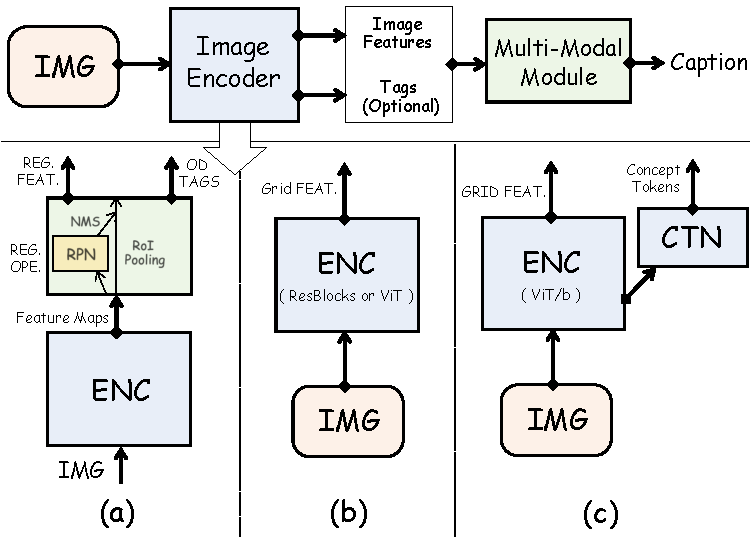
\includegraphics[width=.76\textwidth]{./images/vit_cap.pdf} 
  \end{center}
  \vspace{-5mm}
    \caption[Comparisons of different image captioning models.]{\small \textbf{Comparisons of different image captioning models}. Top: A general image captioning pipeline. Bottom: (a). Prevailing conventional models~\citep{li2019scale,zhang2021multi,hu2020vivo} which are based on an object detector to extract regional features. 
    Object tags~\citep{li2020oscar,zhang2021multi} can be optionally used to assist the text generation through a multi-modal decoder network. This usually requires regional operations (REG. OPE.) that are time consuming.
    (b). To eliminate the detection module, a ResNet variant~\citep{he2016deep} or Vision Transformer~\citep{kim2021vilt} can be applied as substitution to output the grid feature~\citep{xu2021e2e,wang2021simvlm}. 
    This replacement has been studied on the image understanding task recently but very few works
    focus on the generation task. 
    (c). Our proposed \vitcapp\!\!, which is detector-free and incorporates a novel Concept Token Network
    to predict semantic concepts as tokens for the image captioning task.
    }
    \vspace{-2mm}
  \label{fig:abstract}
\end{figure}

Despite these significant advances, most of the mainstream captioning models~\citep{cornia2020meshed,pan2020x,ting2019hierarchy,zhang2021rstnet} rely heavily on a bulky object detector to provide regional visual representations for the multimodal interaction, as shown in Figure~\ref{fig:abstract}-a. 
In spite of the superior performance brought by the object features, 
the ensuing difficulties occur as they: 1) \textbf{lead to heavy computational load} due to the regional operations (\ie, RPN, RoI Pooling, and NMS). These intermediate operations unavoidably cause training inefficiency and high inference latency at prediction stage~\citep{kim2021vilt,wang2020minivlm}; 2) \textbf{require box annotations} and largely limit the flexibility in training and application;  
% 3) are \textbf{unable to update the visual features} from the detector which are not directly optimized towards generating high quality image captions~\citep{xu2021e2e}. 
To address these challenges, there is an emerging trend that more recent works propose to eliminate the detector for the VL pre-training in an end-to-end fashion~\citep{jiang2020defense,huang2020pixel,kim2021vilt,yan2021grid,wang2021simvlm}. In such detector-free design, a general visual encoder serves as a substitute for the detector and from which the grid features are produced for later cross-modal fusion, as in Figure~\ref{fig:abstract}{\color{black}-b}.
Heretofore, the majority of these works mainly focus on the image understanding task, which is typically cast as a classification problem, and only a few of them shed light on the generation task.
In~\citep{xu2021e2e}, the image is encoded with ResNet~\citep{he2016deep} and 
the performance ($117.3$ CIDEr on COCO~\citep{xu2021e2e})
is still far from the state-of-the-art detector-based approach ($129.3$ CIDEr with VinVL-base~\citep{zhang2021multi}).
% with moderate VL training corpus ($6$ million image-text pairs),
% Recent work of SimVLM~\citep{wang2021simvlm} boosts the performance significantly but with as large as $1.8$ billion image-text pairs, which is inaccessible for public. 
% In the meantime, we observe that the currently existing endeavors for the image captioning task are still far from reaching on par outcomes of the detector-based methods, from either the perspective of performance~\citep{xu2021e2e} or training efficacy (\eg, \citep{wang2021simvlm} exploits a massively larger VL corpus than the previous). 
The challenge remains uncharted and insufficiently investigated regarding \textit{how to build a stronger detector-free image captioning model.}
% (\eg, E2E-VLP reaches only $117.3$ CIDEr scores on COCO-caption compared with $123.7$ from~\citep{li2020oscar})


Previous efforts~\citep{li2020oscar,hu2020vivo,zhang2021multi,wang2020minivlm,fang2021compressing} have demonstrated that the object tags play an important role in improving the captioning performance. 
Instead of gleaning the object tags from the detector, we introduce a novel fully \textbf{VI}sion \textbf{T}ransformer based image \textbf{CAP}tioning model, dubbed ViTCAP, with a lightweight Concept Token Network (CTN) that produces concept tokens (see Figure~\ref{fig:abstract}{\color{black}-c}). 
ViTCAP is constructed on the basis of a vision transformer~\citep{dosovitskiy2020image} as the stem image encoder. Our vision transformer backbone starts with encoding the image and produces grid features, on top of which the CTN branch is then applied to predict semantic concepts of images. We represent the semantic concepts at the token level instead of the tag level to avoid the tokenization. 
The multi-modal module then takes the input of both grid representations and Top-$K$ concept tokens for decoding. During training, the CTN is optimized to predict the pseudo ground-truth concepts extracted from image captions via a simple classification task. We also investigate to adopt the object tags from the detector as the pseudo ground-truth, and empirically observe no further improvement. Overall, this straight-forward design allows the injection of semantic concepts into the multi-modal fusion module with abundant semantics, and is critical for the improved captioning performance.

Our ablative analysis suggests that, with no bells and whistles, simple vanilla transformer architecture based \vitcap 1) significantly outperforms existing detector-free captioning models;
%2) surpasses most detector-based models and approaches on par performances with staste of the arts. 
2) surpasses most detector-based models and 3) approaches the state-of-the-art detector-based models. 
% with great inference speed improvement on multiple image captioning benchmarks.
In particular, \vitcap achieves $138.1$ CIDEr scores on COCO-caption Karpathy split~\citep{lin2014microsoft}, $108.6$ on Google-CC~\citep{sharma2018conceptual}, and $95.4$ on nocaps~\citep{agrawal2019nocaps} datasets.

\noindent To summarize our contributions:
\begin{itemize} [leftmargin=8pt]
    \item We present a detector-free image captioning model  \vitcap\!\! with fully transformer architecture, where it leverages grid representations without regional operations. 
    \item We propose to inject semantic concepts into end-to-end captioning by learning from open-form captions. We find that our proposed concept classification training and concept tokens significantly benefit the captioning task.
    \item Extensive evaluations on multiple captioning datasets confirm the validity of our method. \vitcap achieves competitive or even leading results amongst detector-based prior arts with clear inference-time advantages.
\end{itemize}


\subsection{ViTCAP}
% Vision Transformer for Image Captioning
Existing image captioning models usually consist of an object detector module (\textbf{Detector}) to extract regional feature ($\vv^{T}$) from the raw image (\,$\mathbf{I}$\,), and a multi-modal module (\textbf{MM}) to generate a textual description (\,$\vc$\,). Several recent works~\citep{li2020oscar,zhang2021multi} show that the object tags ($\vt^{T}$) extracted from the detector can serve as anchoring points across modalities, and are essential for various VL tasks. This procedure can be expressed as follows:
\begin{equation}
    (\vv^{T}, \vt^{T}) = \text{\textbf{Detector}}(\, \mathbf{I}\,), \cv = \text{\textbf{MM}}(\vv^{T}, \tv^{T}).
\end{equation}
Several VL models~\citep{huang2020pixel,kim2021vilt,xu2021e2e} obtain a great improvement in inference speed by using general image encoders without regional operations. However, these models are unable to utilize the image tags due to the absence of a detector.  

In this work, we aim to build a detector-free captioning model with concept tokens containing rich semantics, coming from a novel Concept Token Network (CTN).
An overview of \vitcap is depicted in Figure~\ref{fig:architecture}. 
The raw image is firstly fed into the image encoder to generate the intermediate representations ($\vv_{i}$) and the final grid representations ($\vv$).
% \vitcap consists of an image encoder module that produces an grid representations ($\vv$),
A CTN branch then takes $\vv_{i}$ as the input and predicts concept tokens ($\tv$), followed by the multi-modal module that allows the interactions across modalities and generates caption ($\cv$). We adopt the fully transformer~\citep{vaswani2017attention} framework in all modules, but the image encoder and CTN modules are not architecture-specific. The overall pipeline can be summarized as:
% \text{\textbf{M}}^{2}\text{-}\, \text{\textbf{Mod.}}
\begin{equation}
    (\!\vv_{i}, \vv\!) \!=\! \text{\textbf{Encoder}}(\, \mathbf{I}\,), \ \ \tv \! = \! \text{\textbf{CTN}}(\vv_{i}), \ \ \cv \! = \! \text{\textbf{MM}}(\vv, \tv).
\end{equation}
In the following, we first introduce how the vision transformer produces grid representations and our proposed CTN in Section~\ref{sec:tagger}, and the overall training losses in Section~\ref{sec:training}.


 
\subsubsection{Model Structure}
% \subsubsection{Vision Transformer}
\noindent \textbf{Vision Transformer.}
\label{sec:vit}   % its okay to release some space here.
The transformer architecture and its instantiations (\eg, BERT~\citep{devlin2018bert}, GPT~\citep{brown2020language}) are well-known for their remarkable performances on natural language processing tasks, which are mostly attributed to the self-attention design. Recent efforts have advanced this to vision tasks, \ie, Vision Transformer (ViT)~\citep{dosovitskiy2020image}. 
We use ViT as the backbone of the image encoder to produce grid representations ($\vv_i$ and $\vv$ ). 
% To be specific, the raw image $\mathbf{I}\in\mathbb{R}^{H\times W \times3}$ is partitioned into $N$ disjoint patches with each in the size of $P\!\times\!P\!\times\!3$, $N\!=\frac{H\times W}{P\times P}$. 
To be specific, the raw image $\mathbf{I}\in\mathbb{R}^{H\times W \times3}$ is partitioned into $N$ disjoint patches. The size of each patch is $P\!\times\!P\!\times\!3$ and the number of patches $N\!$ is 
% $\frac{H\times W}{P\times P}$. 
${(H W)}/{P^2}$. 
% These patches are then flattened and projected into patch embedding of dimension $d$ via a trainable linear projection layer, feeding into consecutive transformer blocks thereafter. 
These patches are then flattened and projected into patch embedding of dimension $d$ via a trainable linear projection layer. Concatenated with a special \texttt{[CLS]} token, these patch representations are added with learnable positional embeddings and then sent into $M$ consecutive transformer blocks thereafter. 
To this end, we use the final representation as the grid features $\vv$, and extract the output of the first $M_1$ blocks as the intermediate representations $\vv_i$, which is the input of the Concept Token Network for concept predictions as detailed below. 
% To this end, grid representations $\vv_i, \vv\in\mathbb{R}^{(N+1)\times d}$ of the image are produced for decoding, with one additional feature for the \texttt{[CLS]} token. $\vv_i$ and $\vv$ are intermediate and final grid representations produced from the stem image encoder and feature extractor.
% The CTN is built upon the initial $M_1$$ transformer blocks with the image encoder (stem image encoder as in Figure~\ref{fig:architecture}), which saves the computational cost with minor performance loss. We experiment with a different number of sharing blocks and compare their results in ablations.
% The intermediate grid representations $\vv_{i}\in\mathbb{R}^{(N+1)\times d}$ are produced from the stem image encoder for the CTN branch. 

\vspace{1mm}
\noindent \textbf{Concept Token Network.}
% \subsection{Concept Token Network}
\label{sec:tagger}
The Concept Token Network (CTN) is composed of $M_2$ transformer blocks to process the intermediate
features $v_i$. The output representation corresponding to \texttt{[CLS]} is used to predict the 
concept token with a multi-linear perceptual (MLP) network. 
The vocabulary of the concept token is identical with the one used for the captions. 
It is noted that we predict the concept in the token level rather than in the tag level, and thus the top-$K$ ($K=50$ in our experiments) tokens can be directly used by the multi-modal decoding module for auto-regressive decoding. In~\citep{li2020oscar,zhang2021multi}, the object tags are predicted from the object detector, while we eliminate the detection module to remove the dependency of the box annotations. Another difference lies in the tag/concept vocabulary. The existing approaches apply the tag list from the dataset as the vocabulary which are pre-defined and need an extra tokenization operation. Instead, our concept token vocabulary is shared with the one for captions and also removes the tokenization step.

% to avoid the 
% tokenization operation. 

% Heretofore, most existing VL models rely on the object detector to retrieve expressive regional features and object tags~\citep{li2020oscar,zhang2021multi} as the anchor points. These categorical tags are known to implicitly align between text and the regional features, thus beneficial for VL tasks. We propose to build a Concept Token Network on top of the stem image encoder, where the CTN predicts semantic concepts through a classification task. In practice, our CTN consists $M-M_1$ transformer blocks to guarantee a consistent 

% We formulate the concept token learning process as a $K$-way classification task using the \texttt{[CLS]} token embedding after a classification head consisting of two linear projection layers. When proceeding to the decoding module, we simply retain the embeddings of the top-$K$ concepts from the vocabulary as concept tokens $\tv$. This exempts us from the operation of tokenization during captioning, and differs from how object tags are encoded as in previous VLP works~\citep{li2020oscar,zhang2021multi}.
% Details of CTN training are discussed in later sections.



\vspace{1mm}
\noindent \textbf{Multi-Modal Fusion Module.}
% \subsection{Multi-modal Module for Decoding}
\label{sec:multimodal}
% Our multi-modal fusion module is a shallow network composed of multiple transformer blocks. 
% % During decoding, we first adopt the Top-$K$ concept tokens' indexes to retrieve their corresponded token embedding from the caption embedding layer as concept token embedding $\tv$. 
% During decoding, the Top-$K$ concept tokens' indexes is mapped to token embeddings through an embedding layer, which is shared with the caption embedding layer.
% Then, the module takes as input the concatenation of concept token embedding and grid representations $(\tv, \vv)$. And during decoding, the multi-modal module produces the caption $\cv$ in an auto-regressive manner given the first \texttt{[CLS]} token. % During decoding, we first adopt the Top-$K$ concept tokens' indexes to retrieve their corresponded token embedding from the caption embedding layer as concept token embedding $\tv$. 
Our multi-modal fusion module is a shallow network composed of multiple transformer blocks, and we follow~\citep{radford2018improving,brown2020language} to apply the \texttt{seq2seq} attention mask to generate the caption token in an auto-regressive way.
First, the Top-$K$ concept tokens' indices are mapped to token embeddings through an embedding layer $l_c$.
Then, the module takes as input the concatenation of concept token embeddings ($\tv$) and grid representations ($\vv$) to generate the description, where we append a mask token \texttt{[MASK]} to the previous generated tokens (empty at very beginning) to predict the next token one by one.
With the \texttt{seq2seq} attention mask, the generated token (including the appended \texttt{[MASK]} token) is able to access the preceding tokens and $(\tv, \vv)$, while $(\tv, \vv)$ has no access to the generated tokens.  
The generated caption token is also mapped through an embedding layer $l_d$.
In experiments, we make the two embedding layers ($l_c$ and $l_d$) shared to reduce the parameter size as the result is similar to two separate layers. 
% Empirically, we observe that the results are similar when $l_c$ and $l_d$ are shared or not (see Appendix for results). To reduce the parameter size, we use the shared embedding layer for both steps. For the auto-regressive decoding, we also have an embedding layer $l_d$ to map the generated token which is shared with the caption embedding layer





\begin{figure*}[t!]
  \begin{center}
    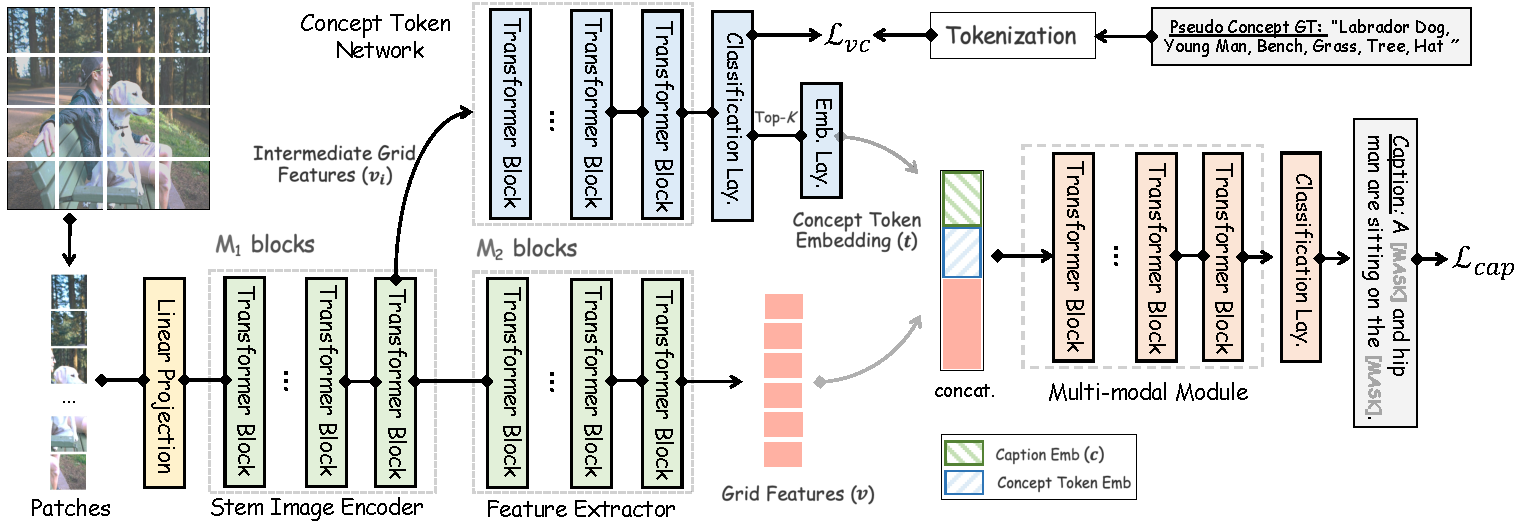
\includegraphics[width=\textwidth, height=0.35\textwidth]{./images/vitcap_architecture.pdf}
    \vspace{-8mm}
  \end{center}
    \caption[Architecture of our proposed \vitcapp image captioning model]{\small \textbf{Architecture of our proposed \vitcapp image captioning model}. \vitcapp is a detector-free image captioning model based on the vision transformer, where image patches are encoded into continuous embeddings as grid representations. The CTN branch roots from an intermediate block of the image encoder, and is a shallow transformer architecture (\eg, 4 self-attention blocks). The CTN is trained via a classification task using object tags gleaned from the Teacher VLM's detector as pseudo-labels and the keywords parsed from image captions as the semantic concept ground-truth. During captioning, the CTN-produced concept tokens from the semantic concept vocabulary are then concatenated with the grid representations and fed into the multi-modal module for decoding. Best viewed in color.
    }
  \label{fig:architecture}
  \vspace{-3mm}
  \end{figure*}

\subsection{Model Training}
\label{sec:training}
The training of \vitcap is composed of the CTN and the captioning training.
% , where the CTN learns to predict existed image-level concepts.
% We jointly optimize both multi-modal module and the TCN branch as the pre-trained TCN can be further adapted at the captioning dataset.
% In order to inject broad semantic concepts into the model, we use the caption extracted keywords (including nouns and adjective words) as the pseudo ground-truth concepts. 
% An alternative way to retrieve the target concepts is to leverage the detector-produced image tags. We also experiment with the object detector pre-trained on Visual Genome~\citep{krishna2017visual} to generate categorical tags as the image-level pseudo-labels for training but find no better results. This is because though such detectors are capable of recognizing diverse collections of semantic concepts, they are largely limited because of the pre-defined categories based on the pre-training dataset. Learning from open-form captions gives much richer concepts, while adopting the detector-produced tags as pseudo-labels allows flexible training when image captions are not attainable. 
CTN is used to predict the image concepts. However, the widely-used VL pre-training dataset contains only the image descriptions without the tags. To address the issue, one can simply retrieve the concepts from the open-form captions (\eg, by extracting nouns or adjective words as keywords) as the pseudo ground-truth concepts, or alternatively leverage a pre-trained object detector (\eg on Visual Genome~\citep{krishna2017visual}) to produce the image tags (remove the bounding boxes). Empirically, we observe that by using caption extracted concepts lead to better results.
% The training of \vitcap is composed of the CTN and the captioning training, where the CTN learns to predict existed image-level concepts.
% % We jointly optimize both multi-modal module and the TCN branch as the pre-trained TCN can be further adapted at the captioning dataset.
% In order to inject broad semantic concepts into the model, we use the caption extracted keywords (including nouns and adjective words) as the pseudo ground-truth concepts. 
% An alternative way to retrieve the target concepts is to leverage the detector-produced image tags. We also experiment with the object detector pre-trained on Visual Genome~\citep{krishna2017visual} to generate categorical tags as the image-level pseudo-labels for training but find no better results. This is because though such detectors are capable of recognizing diverse collections of semantic concepts, they are largely limited because of the pre-defined categories based on the pre-training dataset. Learning from open-form captions gives much richer concepts, while adopting the detector-produced tags as pseudo-labels allows flexible training when image captions are not attainable. 
% we experiment with different sources of semantic concepts as learning targets: 1). the detector-produced image tags, and 2). keywords extracted from the descriptive image captions as target concepts. 
% We leverage the object detector pre-trained on Visual Genome~\citep{krishna2017visual} to generate categorical tags as the image-level pseudo-labels for training. Even though such detectors are capable of recognizing diverse collections of semantic concepts, they are largely limited because of the pre-defined categories based on the pre-training dataset. covering extensive objects and visual attributes. 
% % By concatenating both the object labels and attribute labels as VinVL for a more diverse collection of semantic concepts, covering $1,848$ object categories and $524$ attribute categories. 
% To further broaden the semantic concepts, we expand the taxonomy of semantic concepts by extracting keywords from image captions. Though learning from open-form captions gives much richer concepts, adopting the detector-produced tags as pseudo-labels allows flexible training when image captions are not attainable.
We optimize the CTN to predict the target concepts via a multi-label classification task. Due to the extremely imbalanced semantic concepts distribution (certain concepts appear much frequently than the rest), we adopt the simplified asymmetric focal loss~\citep{ben2020asymmetric,liu2021query2label,lin2014microsoft} which shows great performances handling sample imbalance problems for the multi-label classification task. The overall concept classification loss can be expressed as: 
%  \ \ \  \text{where} \ \
\begin{align}
\mathcal{L}_{{vc}} = \mathbb{E}_{\vv_i\sim D}f_{\theta}(p\ |\ \vv_i),
\end{align}
% and the objective $f_{\theta}(p\ |\ \vv_i)$ is:
\begin{equation}
      f_{\theta}(p\ |\ \vv_i) = \frac{1}{K} \sum^{K}_{k=1}
\begin{cases}
    (1-p_{k})^{\gamma_{+}}\cdot\text{log}(p_k), & +, \\ p_{k}^{\gamma_{-}} \cdot \text{log}(1-p_k), & -,
\end{cases} 
\end{equation}
$p_k \in [0, 1]$ denotes the output probability for the $k$-th class and ${\pm}$ specifies whether the class is the pseudo ground-truth concept. Despite the rarity of positive samples, setting parameters $\gamma_{+} < \gamma_{-}$ decouples its decay rates from the deluge of negative samples and emphasizes more the contribution of the positive. We set parameters $\gamma_{+}=0$ and $\gamma_{}-=1$ as~\citep{liu2021query2label} in our experiment.

% To make the training\&inference consistent, we use unidirectional attention map in our multi-modal module for both phases as a sequence-to-sequence generation task auto-regressively.
% We use unidirectional attention map in our multi-modal module for both phases as a sequence-to-sequence generation task auto-regressively.

For the captioning training, the multi-modal module takes the Caption-Concept Token-Feature triple $(\cv, \tv, \vv)$ as input, 
% where $\cv$ is the caption embedding sequences after tokenization, and $\cv$ is $15\%$ of masked tokens ($\Cv_{M}$) for prediction. 
where $\cv = \{\cv_1, \dots \cv_T\}$ are the masked input words after tokenization and we set the mask probability $=15\%$. The masked tokens are replaced with the special token \texttt{[MASK]}.
% is masked caption embedding sequences after tokenization. The mask rate is $15\%$ and the masked tokens ($\Cv_{M}$) is used for the loss calculation. 
% As inaccurate concept tokens might impose detrimental effects for captioning, we only retain the top-$K$ predicted concepts.
The prediction of masked token at the position $t$ is conditioned on the preceding tokens ($\cv_{<t}$), visual representations ($\vv$) and the concept tokens ($\tv$). We train our model parameters $\theta$ by minimizing the negative log-likelihood over the masked tokens:
\begin{equation}
    \mathcal{L}_{cap} = -\mathbb{E}_{\Tv\sim D}\Big[\text{log}\prod_{\hat{\cv_{t}}\sim \Cv_{M}} P_{\theta}(\hat{\cv_{t}}|\cv_{<t}, \tv, \vv)\Big],
\end{equation}
where $\Cv_{M}$ refers to the ground-truth set of the masked tokens.
% and $\hat{\cv_{t}}$ is the ground-truth token of the masked token $\hat{\cv_{t}}$.

Recent works~\citep{fang2021compressing,liu2021kd} reveal that by leveraging the knowledge distillation technique~\citep{hinton2015distilling}, the VL model can be improved compared to the non-distilled counterpart using a pre-trained Teacher VL model. In our training, we experiment with applying a trained detector-based captioning model as the Teacher (parameterized by $\theta_{t}$), \ie, VinVL~\citep{zhang2021multi}, to assist the training of \vitcap\!\!. Note that the Teacher model is a two-stage VL model adopting regional features and object tags from the detector, yielding discrepant visual features with \vitcap\!\!, and hence the distillation objectives like attention-map loss and hidden-states loss are not directly applicable as in~\citep{fang2021compressing}. We adopt the classification distillation loss over the masked token probabilities between the predictions from the Student ($P_\theta$) and Teacher ($P_{\theta_t}$) models:
\begin{equation}
    % \mathcal{L}_{dis} = \mathbb{E}_{(\Tv, \Tv_{t})\sim D}\Big[\text{log}\!\!\!\!\prod_{\hat{\cv_{t}}\sim \Cv_{M}}\!\!\!\! f_{\theta}(\hat{\cv_{t}}|\cv_{<t}, \tv, \vv, \tv_{t}, \vv_{t}, \theta_{t})\Big],
    \mathcal{L}_{dis} = \mathbb{E}_{\Tv\sim D}\Big[\sum_{\hat{\cv_t}\sim\Cv_{M}}\text{KL}{\Big(}P_\theta(\hat{\cv_t}), P_{\theta_t}(\hat{\cv_t}){\Big)}\Big],
\end{equation}
where KL$( \ , \ )$ is the Kullback–Leibler divergence.
% where $f_{\theta}(\,\cdot\,|\,\cdot\,) = \textsc{CE}(\mathbf{z}/\tau, \mathbf{z}_{ t}/\tau)$ and $\tau$ denotes the temperature parameter set as constant $\mathds{1}$, and $\mathbf{z}$, $\mathbf{z}_{t}$ refer to the predicted token probabilities from Student and Teacher respectively. 
Overall, our final loss is then the combination of the terms:
\begin{equation}
    \mathcal{L} = \mathcal{L}_{vc} + \mathcal{L}_{cap} + \mathcal{L}_{dis}.
\end{equation}
% $\lambda$ is a hyper-parameter weighting the loss terms. 
% We discuss more training details in the later section.
% , and we find satisfactory results by setting  $\lambda = 10$ in our experiment.

\subsection{Experiment}
We now introduce the implementation details of \vitcap and empirically verify the validity of our proposed training schema from different aspects. 
To highlight the generalizability of \vitcap\!\!, we benchmark performances of \vitcap and compare it with prior arts on multiple image captioning testbeds. We then exhaustively study the effect of our proposed concept tokens, the benefits of pre-training at scale, the effect of VL distillation, \etc. In the end, we visualize the attention maps of \vitcap and provide in-depth discussion. 


\subsubsection{Datasets}

\vspace{1mm}
\noindent \textbf{Pre-training Datasets.}
% VL pre-training has shown great performances on multiple VL-related tasks, \eg, image captioning, VQA, and retrieval. 
In our experiment, we aggregate image-text pairs from Google-CC~\citep{sharma2018conceptual}, SBU Caption dataset~\citep{ordonez2011im2text}, MS COCO~\citep{lin2014microsoft} and Visual Genome dataset~\citep{krishna2017visual} to form the pre-training corpus.  In total, our pre-training corpus contains $9.9$M image-text pairs and $4.1$M independent images, and we follow~\citep{lu202012} to de-duplicate testing images exist in evaluating datasets. Details of the pre-training corpus can be found in later section. 
% Unlike most VL pre-training works that use image-text pairs matching loss and unidirectional masked token loss as the training loss, we find that a consistent pre-training training objective as in the downstream task leads to better performances. 
% Thus our pre-training paradigm follows the identical training loss as introduced in Section~\ref{sec:training}.

\vspace{1mm}
\noindent \textbf{Evaluation Datasets.}
% \footnote{\url{https://github.com/karpathy/neuraltalk2}.}
We report performances of \vitcap on {{COCO captions}} (Karpathy split)~\citep{lin2014microsoft}, {{Google-CC}}~\citep{sharma2018conceptual}, and {{nocaps}}~\citep{agrawal2019nocaps} datasets. We follow Karpathy’s split and use~$113$k, $5$k and $5$k images for training, validation and testing respectively on MS COCO dataset. As regards to Google-CC, we follow~\citep{sharma2018conceptual} and use its training split containing~$3$M image-text pairs for training, and report the performances on validation split with~$16$K image-text pairs. To test the generalization of \vitcap\!\!, we also report the performances on nocaps dataset~\citep{agrawal2019nocaps}, a benchmark consisting of $166$k human-generated captions describing $15$k images in the wild collected from the OpenImages dataset~\citep{shao2019objects365}. 



\subsubsection{Implementation Details}
\vspace{1mm}
\noindent \textbf{Architecture.}
Our \vitcap is based on a Vision Transformer base (ViT/b) architecture consisting of $M=12$ consecutive transformer blocks, with hidden size as $768$, and $12$ attention heads. In our experiment, we set the patch size as $16 \times 16$ and resize the shorter side of the image to $384$. We use $M_1=8$ transformer blocks in Stem Image Encoder to extract the intermediate grid representations and use $M_2=4$ transformer blocks for the CTN branch.
Data augmentations are applied on raw images before the linear projection as~\citep{dosovitskiy2020image} including \textit{ColorJitter}, \textit{horizontal flipping}, \etc.

\vspace{1mm}
\noindent \textbf{Two-stage Training.}
Training both the CTN branch jointly with the captioning task jointly from scratch is challenging, we observe that using a pre-trained CTN with stable and consistent concept prediction throughout the training leads to superior captioning results. Thus in practice, we first conduct concept classification training for a good concept prediction, and then train the model with both tasks. 
Such strategy prevents the ``\textit{cold-start}'' issue when the initially produced concepts are mostly random, impairing the captioning training. During the joint captioning \& concept branch training, we reduce the learning rate for both the Stem Image Encoder and CTN branch by a factor of $\alpha$ ($\alpha = 10$) and keep the predicted concepts relatively consistent but still slowly adapted throughout the training. 
\vspace{-2mm}
\begin{itemize} [leftmargin=8pt]
    \item \textbf{Concept Classification.} The concept classification is conducted on an aggregated dataset with $4.1$M images (see later section for details). To obtain the pseudo ground-truth concepts, we experiment with using the NLTK~\citep{loper2002nltk} toolkit to parse out the nouns and adjectives as the target concepts, or simply use all tokens in captions as targets for the classification task. For the detector-produced tags, we take advantage of a ResNeXt-$152$ C4 architecture based object-attribute detector that has been well-trained~\citep{zhang2021multi} to produce image tags as pseudo-labels for concept classification training. We only retain image tags with confidence score $> 0.2$ from the detector and acquire $50$ tags at most per image. For classification training, the model is initialized from the ImageNet-$21$k~\citep{krizhevsky2012imagenet} pre-trained checkpoint\footnote{\url{https://github.com/lucidrains/vit-pytorch}.}, and is optimized for $10$ epochs using AdamW~\citep{you2019large,reddi2019convergence} optimizer. The batch size is $1,024$. The initial learning rate is $5e-5$ and is linearly decayed to $0$. 
    \vspace{-2mm}
    \item  \textbf{Captioning Training.} For the joint optimization, we apply the well-trained model after concept classification to initialize Stem Image Encoder, CTN and the feature extractor. The initial weights in the feature extractor are copied from the CTN branch, as the architecture for grid feature extractor is the same as the CTN branch. We set base learning rate~$lr=1e-4$, batch-size $=512$ and train the model for $30$ epochs using AdamW optimizer, and set weight decay$=0.05$. 
\end{itemize}
% \vspace{1mm}
\noindent \textbf{Evaluation.} We evaluate the quality of the generated captions using the prevailing metrics including BLEU@$4$~\citep{papineni2002bleu}, METEOR~\citep{banerjee2005meteor}, CIDEr~\citep{vedantam2015cider}, ROUGE~\citep{lin2004rouge} and SPICE~\citep{anderson2016spice}. During inference, we use beam search (beam size $= 1$) for decoding.


% COCO_Captioning Results
\begin{table*}[t] 
\small
\centering
\renewcommand{\arraystretch}{1.1} 
\vspace{-1mm}
\setlength\tabcolsep{9.2pt}
\caption[Performance comparisons on \coco Karpathy split.]{\small Performance comparisons on \coco Karpathy split, where B@$4$, M, R, C denote BLEU@$4$, METEOR, ROUGE-L, CIDEr and SPICE scores. All values are reported as percentages (\%). We compare the \vitcap with previous state-of-the-art detector-based baselines (without the VLP) in the first section, and detector-based baselines (with large scale pre-training) in the third section, and the detector-free methods with pre-training in the last section.
V. ENC. denotes visual encoders for feature extraction; \# \textit{I-T} refers to the number of image-text pairs used in pre-training (in millions). 
$^{\color{black}{\spadesuit}}$ is the results we achieved using the VILT~\citep{kim2021vilt} pre-trained checkpoint for image captioning task. 
$^{\color{black}{\heartsuit}}$ is the result using concepts from captions.
}
% \vspace{-2mm} c@{\vline}
\scalebox{.6}{
% \begin{tabular}{p{24mm} c p{9mm}  c c c c  c | c c c c c}
\begin{tabular}{p{24mm} c p{9mm}  c c c c  c c c c c c}
\toprule
 \\[-2.5ex]
\multirow{2}{*}{\textbf{Methods}} & \multirow{2}{*}{V. ENC.} & \multirow{2}{*}{\# \textit{I-T}} & \multicolumn{5}{c}{{\texttt{\textbf{Cross-Entropy Loss}}}} & \multicolumn{5}{c}{{\texttt{\textbf{CIDEr Optimization}}}} \\
\cmidrule(r){4-8} \cmidrule(l){9-13}
&  &  & \multicolumn{1}{c}{B@4 } & M    & R    & C     & \multicolumn{1}{c}{S}  &  B@4  & M  & R  & C     & S  \\	\hline \\[-2ex]
{$^{{\color{black}{\text{\textbf{Detector}}}}\text{ w.o. }\color{black}{\text{\textbf{VLP}}}}$} & & & & & & & & & \\[-6pt]
{\cellcolor{black!3} RFNet}       & Ensemble & \ \ \xmarkg & $35.8$ & $27.4$ & $56.5$ & $112.5$ & $20.5$ & $36.5$ & $27.7$ & $57.3$ & $121.9$ & $21.2$ \\
{\cellcolor{black!3}BUTD}    & F-RCNN$_{101}$ & \ \ \xmarkg & $36.2$ & $27.0$ & $56.4$ & $113.5$ & $20.3$ & $36.3$ & $27.7$ & $56.9$ & $120.1$ & $21.4$ \\
{\cellcolor{black!3}LBPF}        & F-RCNN$_{101}$ & \ \ \xmarkg & 37.4 & 28.1 & 57.5 & 116.4 & 21.2 & 38.3 & 28.5 & 58.4 & 127.6 & 22.0 \\
{\cellcolor{black!3}SGAE}        & F-RCNN$_{101}$ & \ \ \xmarkg & $36.9$ & $27.7$ & $57.2$ & $116.7$ & $20.9$ & $38.4$ & $28.4$ & $58.6$ & $127.8$ & $22.1$ \\
{\cellcolor{black!3}AoANet}      & F-RCNN$_{101}$ & \ \ \xmarkg & $37.2$ & $28.4$ & $57.5$ & $119.8$ & $21.3$ & $38.9$ & $29.2$ & $58.8$ & $129.8$ & $22.4$ \\
{\cellcolor{black!3}M$^{2}$ Transfm.} & F-RCNN$_{101}$ & \ \ \xmarkg & - & - & - & - & - & $39.1$ & $29.2$ & $58.6$ & $131.2$ & $22.6$\\ 
{\cellcolor{black!3}X-LAN}       & F-RCNN$_{101}$ & \ \ \xmarkg & $38.2$ & $28.8$ & $58.0$ & $122.0$ & $21.9$  & $39.5$ & $29.5$ & $59.2$ & $132.0$ & $23.4$ \\
{\cellcolor{black!3}RSTNet} & RESNeXt$_{152}$ & \ \ \xmarkg & - & - & - & - & - & $40.1$ & $29.8$ & $59.5$ & $135.6$ & $23.3$\\ 
\hline \\[-2ex]
{$^{{\color{black}{\text{\textbf{Detector-Free}}}}\text{ w.o. }\color{black}{\text{\textbf{VLP}}}}$} & & & & & & & & & \\[-6pt]
{\cellcolor{black!3}ViTCAP \ \ \ (Ours)}    & ViT$_{b}$  & \ \ \ \xmarkg & $35.9$ & $28.6$  & $57.6$ & $121.3$ & $21.9$ & $40.1$ & $29.4$ & $59.4$ & $133.1$ & $23.0$ \\
{\cellcolor{black!3}ViTCAP$^{\heartsuit}$ (Ours)}    & ViT$_{b}$  & \ \ \ \xmarkg & $36.1$ &  $28.8$ &  $57.6$ & $122.2$ &  $22.1$ & $40.3$ & $29.4$ & $59.5$ & $133.6$ & $23.3$\\
\hline \\[-2ex]
{\cellcolor{black!3}$^{{\color{black}{\text{\textbf{Detector}}}}\text{ w. }\color{black}{\text{\textbf{VLP}}}}$}  &  &  &  &  &  &  & & & & \\[-6pt]
{\cellcolor{black!3} UVLP}        & F-RCNN$_{101}$ & \ $4$M & $36.5$ & $28.4$ & - & $116.9$ & $21.2$ & $39.5$ & $29.3$ & - & $129.3$ & $23.2$ \\
{\cellcolor{black!3} MiniVLM}      & Eff-DET & $14$M & $35.6$ & $28.6$ & - & $119.8$ & $21.6$ & $39.2$ & $29.7$ & - & $131.7$ & $23.5$ \\
{\cellcolor{black!3}DistillVLM}   & Eff-DET & \ $7$M & $35.6$ & $28.7$ & - & $120.8$ & $22.1$ & - & - & - & - & - \\
{\cellcolor{black!3} OSCAR$_\text{b}$}        & F-RCNN$_{101}$ & \ $7$M & $36.5$ & $30.3$ & - & $123.7$ & $23.1$ & $40.5$ & $29.7$ & - & $137.6$ & $22.8$ \\
{\cellcolor{black!3}UNIMO$_\text{b}$} & F-RCNN$_{101}$ & \ $9$M & $38.8$ & - & - & 124.4  & - & - & - & - & - & -\\ 
{\cellcolor{black!3}VL-T5} & F-RCNN$_{101}$ & \ $9$M & - & - & - &  $116.5$ & - & - & - & - & - & -\\
{\cellcolor{black!3}VinVL$_\text{b}$}        & RESNeXt$_{152}$ & \ $9$M  & $38.2$ & $30.3$ & - & $129.3$ & $23.6$ & \textbf{$40.9$} & \textbf{$30.9$} & - & \textbf{$140.4$} & \textbf{$25.1$} \\
\hline \\[-2ex]
{$^{{\color{black}{\text{\textbf{Detector-Free}}}}\text{ w. }\color{black}{\text{\textbf{VLP}}}}$} & & & & & & & & & & \\[-6pt]
% Jacob_Kim_Vilt_captioning_testing_batch-size_512_encoder_vit_base_patch32_384_lr_5e-5_iter_30_with_VLP_  \multirow{3}{*}{\xmark}
{\cellcolor{black!3}ViLT-CAP$^{\color{black}{\ \spadesuit}}$}  & ViT$_{b}$ & \ $10$M & $33.7$ & $27.7$ & $56.1$ & $113.5$ & $20.9$ & - & - & - & - & - \\
{\cellcolor{black!3}E2E-VLP} & ResNet$_{50}$ & \ \ $6$M & $36.2$ & - & - & $117.3$ & - & - & - & - & - & - \\
% SimVLM$_\text{b}$ & ResBlocks & $1.8$B & $\textbf{32.9}$ & - & $134.8$ & $24.0$ & - & - & - & - & - & $39.0$  \\ 
% \vitcap   & \xmark & \xmark & 36.1 & 28.5 & 57.5 & 121.0 & 22.0 & - & - & - & - & - \\
% \cellcolor{red!3}CAPTION$^{\spadesuit}$ & \cellcolor{gray!35}$35.9$ & $28.6$  & $57.6$ & \cellcolor{gray!40}$121.3$ & $21.9$ \\
{\cellcolor{black!3}ViTCAP \ \ \ (Ours)} & ViT$_{b}$  & \ $10$M & $\textbf{36.3}$ & $\textbf{29.3}$ & $\textbf{58.1}$ & $\textbf{125.2}$ & $\textbf{22.6}$ & $\textbf{41.2}$ & $\textbf{30.1}$ & $\textbf{60.1}$ & $\textbf{138.1}$ & $\textbf{24.1}$\\
\bottomrule
\end{tabular}
}
\label{tab:COCO}
\end{table*}


\subsubsection{Main Results}
We perform extensive comparisons of \vitcap with the prior arts. Table~\ref{tab:COCO} presents the captioning results on MS COCO dataset where the models are trained with cross-entropy loss or optimized with CIDEr as reward~\citep{rennie2017self}. 
% Unless specifically noted, 
We compare \vitcap with 1). ``\textit{detector w/o VLP}'' models with complex architectural modifications. These models ~\citep{huang2019attention,cornia2020meshed,pan2020x,zhang2021rstnet} all come unanimously with heavy computational burdens and extra learnable parameters. 2). ``\textit{detector w. VLP}'': prevailing detector-based VL models pre-trained with a large VL corpus and then fine-tuned on image captioning tasks. 3). ``\textit{detector-free}'' methods: the end-to-end trainable image captioning models without object detector (with or without pre-training).


% \vspace{-4mm}
\noindent \textbf{Without VLP.} To compare fairly with the detector-based baselines without VLP,  we adopt the VinVL tags as concept sources instead of the captions to guarantee that \emph{no additional captions have been exploited} during the concept classification training. Note that the knowledge distillation objective is not applied for this experiment as it introduces extra knowledge from the pre-training of Teacher model.
On COCO-caption Karpathy split, our \vitcap achieves similar results and even surpasses most existing detector-based methods, \ie, CIDEr score $121.2$. Using caption extracted concepts leads to better result: \ie, CIDEr score $122.2$.  It is worth mentioning that the architectures of most existing detector-based methods are deliberately designed, \eg, the self-attention module in X-LAN~\citep{pan2020x} has 2$^{nd}$ interactions for multimodal inputs, M$^{2}$ Transformer~\citep{cornia2020meshed} has the multi-level representation of the relationships between image regions, \etc. \vitcap adopts the simplest vanilla transformer architecture without any bells and whistles. This proves the effectiveness of our proposed learning paradigm. 
% It is worth pointing out that we pre-train a ViT/b architecture as the CTN on the $9$M VL corpus and then adapt it for the captioning task by applying its initialization. 
The ablations in the later section comprehensively explore the benefits of CTN and the knowledge distillation technique. 


% \vspace{1mm}
\noindent \textbf{With VLP.}
We observe a clear performance gain of \vitcap after the large scale pre-training ($3.0$ higher CIDEr scores), better than most detector-based VL methods: \eg, $125.2$ \vs $123.7$ (OSCAR$_{b}$), and $0.8$ higher than UNIMO$_{b}$, $8.7$ higher than VL-T$5$ when pre-trained on similar VL corpus. This conclusion is further supported by results of other metrics. \vitcap approaches the state of the art, only $2.3$ lower than VinVL in CIDEr scores after CIDEr optimization, considering the fact that VinVL used ResNeXt$_{152}$-based object detector.
% \vitcap approaches comparable performances with the state of the art, only $2.3$ lower than VinVL$_{b}$ CIDEr scores after CIDEr optimization, regardless of the ResNeXt$_{152}$ based bulky object detector used by VinVL.
Compared with detector-free baselines, \vitcap outperforms all existing works with an obvious discrepancy: $11.5$ CIDEr scores higher than the VILT-CAP~\citep{kim2021vilt} and $7.7$ higher than E2E-VLP~\citep{xu2021e2e}. 

% \vspace{}
In Figure~\ref{fig:flops}, we present the inference speed and the number of learnable parameters of prevailing detector-based VL models compared with \vitcap\!\!. Notably, with on-par parameters, \vitcap consumes only $\sim10\%$ FLOPs of the prevailing VL models ($97$G for \vitcap \vs  $1,025$G for VinVL).

\subsubsection{Ablative Study}
We now comprehensively study \vitcap\!'s performance gain from different aspects, \ie, knowledge distillation, the effect of concept tokens, and large-scale pre-training.
% We conduct and report the results on COCO caption (Karpathy split) dataset. 
% \footnote{We list more ablations regard the effect of concept classification loss, results using architectural variations in the Appendix. }


\begin{figure}[t]
    \centering
  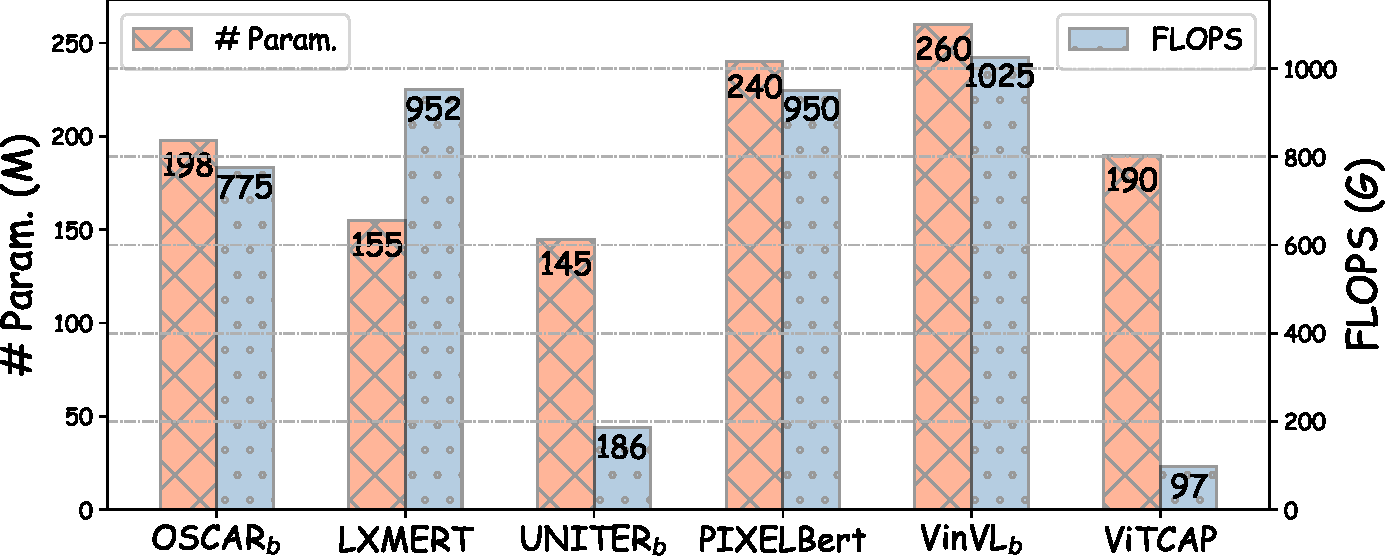
\includegraphics[width=.78\textwidth]{images/flops.pdf}
    \caption {\small Inference speed in FLOPs (in G), number of parameters (in M) of multiple VL models and \vitcapp\!\!.}
    \vspace{-1mm}
\label{fig:flops}
\end{figure}





% Table for semantic concepts
\begin{table}[t]
\centering
\renewcommand{\arraystretch}{1.15} 
\setlength\tabcolsep{8.5pt}
\caption[Adopting various sources of semantic concept leads to different performances.]{\small Adopting various sources of semantic concept leads to different performances. ``CAPTION'' represents the baseline extracting keywords from open-form captions; ``$^{\spadesuit}$'' is the baseline using all words in captions as target concepts; ``BUTD'' and ``VinVL'' represent using the object tags produced by the object detector from~\citep{anderson2018bottom} and~\citep{zhang2021multi} as target semantic concepts, respectively. ``VinVL $\rightarrow$ CAP.'' represents adopting detector tags~\citep{zhang2021multi} during first stage of concept classification and using caption extracted tags during the second stage.}
\scalebox{1.0}
{
\small
\begin{tabular}{p{42mm} | c c c c c }
\toprule
\multirow{2}{*}{\textbf{Concept Source}} & \multicolumn{4}{c}{{ \texttt{\textbf{\ \ \ \ \ COCO Captioning}}}}  \\ 
 & {B@4} & {\ \ M} & {\ \ R} & {\ \ C} & {\ \ S} \\
\hline
\cellcolor{black!3}\xmarkg  & \cellcolor{black!5}$33.9$ & $27.8$ & $56.4$ & \cellcolor{black!5}$114.8$ & $21.3$ \\
\cellcolor{red!3}BUTD & \cellcolor{black!15}$35.0$ & $28.2$ & $56.9$ & \cellcolor{gray!25}$117.4$& $21.3$ \\
\cellcolor{red!3}VinVL  & \cellcolor{black!25}$35.6$ & $28.6$ & $57.4$ & \cellcolor{gray!35}$119.7$ & $21.8$ \\
\cellcolor{red!3}CAPTION & \cellcolor{black!35}$35.6$ & $28.7$  & $57.6$ & \cellcolor{gray!35}$120.9$ & $21.8$ \\
\cellcolor{red!3}VinVL $\rightarrow$ CAP.$^{\spadesuit}$& \cellcolor{gray!35}$35.9$ & $28.6$  & $57.6$ & \cellcolor{gray!40}$121.3$ & $21.9$ \\
\cellcolor{red!3} CAPTION$^{\spadesuit}$ & \cellcolor{gray!45}$36.1$ & $28.8$ & $57.6$ & \cellcolor{gray!45}$122.2$ & $22.1$ \\ 
\bottomrule
\end{tabular}
}
\label{tab:tags}
\end{table}




\vspace{1mm}
\noindent \textbf{Semantic Concept Sources.} We study the effects of different semantic concept sources, \ie, from object detectors~\citep{anderson2018bottom,zhang2021multi}, captions-extacted concepts, and the combination of them. Table~\ref{tab:tags} lists the performances of \vitcap on the COCO caption dataset with various semantic concepts sources. 
Open-form captions are the most accessible source to directly obtain semantic concepts, although these descriptions can sometimes be noisy, inaccurate and incomplete. ``CAPTION'' in Table~\ref{tab:tags} is the result using nouns and adjectives parsed from captions using NLTK~\citep{loper2002nltk} toolkit as target concepts. This leads to an obvious improvement over the baseline (without CTN): CIDEr $120.9$ \vs $114.8$. 
We also attempt to leverage all tokens from the captions as concept targets in case of omitting essential words during parsing (see ``CAP.$^{\spadesuit}$''), which brings further incremental improvement and yield best result. Although using all tokens in the caption might inevitably introduce more noisy or irrelevant words, \eg, connection and stop words, it also broadens the semantic concepts vocabulary as some rare entities/attributes might be missed using just keywords. 
% Refer to the Appendix for more experimental setup details.

\begin{table}[t]
    \centering
    \renewcommand{\arraystretch}{1.2} .
    \caption[Comparisons of \vitcapp with or without knowledge distillation.]{\small Comparisons of \vitcapp with or without knowledge distillation, large-scale pre-training and with CTN. Performances are reported on COCO-caption Karpathy split optimized by cross-entropy loss. $_{+ \text{OD-TAG}}$ indicates the result using the detector produced off-the-shelf tags as~\citep{li2020oscar}. $_{+ \text{CTN-TOK}}$ is the result of \vitcapp using the initialization after first-stage concept classification. $_{\color{darkred}{\text{\textbf{KD}}}}$ and $_{\color{darkgreen}{\text{\textbf{PRE}}}}$ are results obtained with masked token classification distillation and pre-training at scale respectively.
    }    
    \scalebox{0.95}
    {\small
    \begin{tabular}{p{43.5mm} c c c c c }
    \toprule
    \\[-3.5ex]
   \multirow{2}{*}{\textbf{Methods}} & \multicolumn{4}{c}{{\texttt{\textbf{\ \ \ \ Cross-Entropy Loss}}}} \\
    & \multicolumn{1}{c}{B@4 } & M & R  & C     & \multicolumn{1}{c}{S}    \\	
    \hline
    \cellcolor{red!3}ViT/B&   \cellcolor{gray!5}$33.9$ & $27.8$ & $56.4$ &  \cellcolor{gray!5}$114.8$ & $21.3$ \\
    \cellcolor{red!3}ViT/B${\tiny  \scalebox{1.1}{+} \  \color{darkred}{\text{\textbf{KD}}}}$ &   \cellcolor{gray!20}$35.4$ & $28.5$ & $57.5$ & \cellcolor{gray!40}$120.0$ & $21.7$   \\
    \cellcolor{red!3}ViT/B${\tiny \scalebox{1.1}{+} \ \text{CTN-TAG}}$ &    \cellcolor{gray!15}$35.2$ &  $28.0$ & $57.0$ &	\cellcolor{gray!25}$117.1$ & $21.4$ \\
    \cellcolor{red!3}ViT/B${\tiny \scalebox{1.1}{+} \ \text{OD-TAG}}$ &    \cellcolor{gray!10}$34.3$ &  $28.2$ & $57.4$	& \cellcolor{gray!25}$117.4$ & $21.7$\\
    \cellcolor{red!3}ViTCAP${\tiny \scalebox{1.1}{+} \ \text{CTN-TOK}{\color{black}}}$ &    \cellcolor{gray!25}$36.1$ &  $28.8$ & $57.6$	& \cellcolor{gray!35}$122.2$ & $22.1$\\
    % ViTCAP${\tiny \scalebox{1.1}{+} \ \text{VC-TOK} \scalebox{1.1}{+} \ {\color{darkred}{\text{\textbf{KD}}}}  }$ \\
    \cellcolor{red!3}ViTCAP${\tiny \scalebox{1.1}{+} \ \text{CTN-TOK}  \scalebox{1.1}{+} \ {\color{ddarkgreen}{\text{\textbf{PRE}}}} \scalebox{1.1}{+} {\color{darkred}{\text{\textbf{KD}}}} }$ &  \cellcolor{gray!35}$36.3$ &  $29.3$ & $58.1$ & \cellcolor{gray!45}$125.2$ & $22.6$   \\
    \bottomrule
    \end{tabular}
    }
  \label{tab:ablation}
\end{table}
% We also resort to different object detectors to acquire high-quality semantic concepts, \ie, a ResNet$_{101}$ base Faster-RCNN~\citep{anderson2018bottom} that has been pre-trained on Visual-Genome dataset~\citep{krishna2017visual} (denoted as BUTD), and a ResNext$_{152}$ based modified Faster-RCNN detector with broader categories of the visual attribute as detection targets (denoted as VinVL). Although these detector-produced image-level tags are rather accurate with less noise, they require a pre-defined categorical dictionary with a fixed set of vocabulary. We first extract these tags as off-the-shelf annotations for the classification task on a ViT/B model and apply it as the initialization of \vitcap for captioning training. Note that we conduct and compare all these ablations without pre-training. We showcase some qualitative examples with the produced image-level semantic concepts in the Appendix.
We then experiment with using the detectors in~\citep{zhang2021multi} and~\citep{anderson2018bottom} to produce image-level tags as target concepts. We observe that using the detector of VinVL yields better performances than BUTD, \ie, $119.7$ \vs $117.4$ CIDEr scores. This is mainly because of the more diverse collection of semantic concepts involved in~\citep{zhang2021multi} than BUTD~\citep{anderson2018bottom}. 
% including $1,848$ object labels and $524$ attribute labels involved in detection training. 
% Noticeably, direct learning from the caption-extracted keywords leads to better results and by using all tokens as target concepts (denoted CAPTION$^{\spadesuit}$). 
The second last row is the experiment where the model is firstly trained using VinVL tags on large scale dataset (in the first stage), and then using the caption tokens during the second stage of captioning. This indicates that, when no captions are attainable, it is also viable to leverage detector-produced tags to improve the performance.
% This suggests that the extracted concepts enrich the vocabulary and therefore produce tokens with more semantics for the captioning task. 
% This also largely alleviates the challenge where the semantic concepts in the target domain are in different forms \textit{w.r.t.} the source domain descriptions. For example, synonym, cognate and conjugate words or various tenses.


\begin{table}[t!]
\centering
\renewcommand{\arraystretch}{1.05} % Default value: 1
\caption[Performances of \vitcapp model on Conceptual Captions (Google-CC 3M dev-split)~\citep{sharma2018conceptual} benchmark.]{\small
Performances of \vitcapp model on Conceptual Captions (Google-CC 3M dev-split)~\citep{sharma2018conceptual} benchmark. We compare with the baseline methods FRCNN~\citep{changpinyo2019decoupled}, Ultra~\citep{changpinyo2019decoupled} and~\citep{changpinyo2021conceptual}. The ViLT-CAP$^{\color{black}{\spadesuit}}$ and VinVL represent our reproduced results with pre-trained checkpoint from~\citep{kim2021vilt} and~\citep{zhang2021multi}.
}
\scalebox{0.99}
{ 
\small
\begin{tabular}{l|c}
\toprule
\multirow{2}{*}{\textbf{Methods}}  & \multicolumn{1}{c}{{ \texttt{\textbf{CC-3M dev}}}}  \\ 
& {CIDEr} \\
\hline 
   \cellcolor{red!3}FRCNN & $89.2$ \\
   \cellcolor{red!3}Ultra & $93.7$ \\ 
   \cellcolor{red!3}VILT-CAP$^{\color{black}{\spadesuit}}$ & $83.8$\\ 
   \cellcolor{red!3}VinVL$^{\color{black}{\spadesuit}}$ & $103.4$ \\ 
   \cellcolor{red!3}CC-$3$M & $100.9$ \\
   \cellcolor{red!3}CC-$12$M & $105.4$ \\ 
   \hline
   \cellcolor{blue!3}ViTCAP  &  $\textbf{108.6}_\text{\color{darkgreen}\textbf{ +3.2}}$ \\
\bottomrule
\end{tabular}
}
\label{tab:googlecc}
\end{table}


\begin{table}[t!]
    \centering
    \setlength{\tabcolsep}{6pt} % Default value: 6pt
    \renewcommand{\arraystretch}{1.05} % Default value: 1
    \caption [Performances of \vitcapp in nocaps validation split.]{\small Performances of \vitcapp in nocaps validation split. We compare our \vitcapp with previous state-of-the-art models at \textbf{``in-domain''}, \textbf{``near-domain''} and \textbf{``out-of-domain''}. Results are reported with constrained beam search (CBS) decoding~\citep{anderson2016guided}.}    
    \scalebox{0.88}
    {
     \small
    \begin{tabular}{l|cc|cc|cc|cc}
    \toprule
    & \multicolumn{8}{c}{\texttt{\textbf{nocaps validation set}}} \\
    \cline{2-9} 
    \multicolumn{1}{l|}{\textbf{Methods}} & \multicolumn{2}{c|}{\textbf{in-domain}} & \multicolumn{2}{c|}{\textbf{near-domain}} &  \multicolumn{2}{c|}{\textbf{out-of-domain}} & \multicolumn{2}{c}{\textbf{overall}}\\ 
     & C & S & C &  S  & C & S & C & S \\ 
    \hline 
    \transparent{0.4}Human & \transparent{0.4}84.4 & \transparent{0.4}\textbf{14.3} & \transparent{0.4}85.0 & \transparent{0.4}\textbf{14.3} & \transparent{0.4}\textbf{95.7} & \transparent{0.4}\textbf{14.0} & \transparent{0.4}87.1 & \transparent{0.4}\textbf{14.2} \\
    \hline
    \cellcolor{red!3}UpDown & $78.1$ & $11.6$ & $57.7$ & $10.3$ & $31.3$ & $8.3$ & $55.3$ & $10.1$ \\
    \cellcolor{red!3}UpDown + CBS  & $80.0$ & $12.0$ & $73.6$ & $11.3$ & $66.4$ & $9.7$ & $73.1$ & $11.1$ \\
    \cellcolor{red!3}UpDown + ELMO + CBS  & $80.0$ & $12.0$ & $73.6$ & $11.3$ & $66.4$ & $9.7$ & $73.1$ & $11.1$ \\
    % UpDown~\citep{agrawal2019nocaps} + ELMo + CBS & $79.3$ & $12.4$ & $73.8$ & $11.4$ & $71.7$ & $9.9$ & $74.3$ & $11.2$ \\ 
    % UpDown~\citep{agrawal2019nocaps}& $79.3$ & $12.4$ & $73.8$ & $11.4$ & $71.7$ & $9.9$ & $74.3$ & $11.2$ \\ 
    % \hline
    % Oscar$_L$~\citep{li2020oscar} & 79.9 & 12.4 & 68.2 & 11.8 & 45.1 & 9.4 & 65.2 & 11.4 \\
    \cellcolor{red!3}OSCAR & $79.6$ & $12.3$ & $66.1$ & $11.5$ & $45.3$ & $9.7$ & $63.8$ & $11.2$ \\
    \cellcolor{red!3}OSCAR + CBS & $83.4$ & $12.0$ & $81.6$ & $12.0$ & $77.6$ & $10.6$ & $81.1$ & $11.7$ \\
    % Oscar$_L$ + CBS & 78.8 & 12.2 & 78.9 & 12.1 & 77.4 & 10.5 & 78.6 & 11.8 \\
    % OSCAR$_\text{L}$~\citep{li2020oscar}& $85.4$ & $11.9$ & $84.0$ & $11.7$ & $80.3$ & $10.0$ & $83.4$ & $11.4$ \\ 
    % \hline
    % VIVO~\citep{hu2020vivo} & 88.8 & 12.9 & 83.2 & {12.6} & 71.1 & 10.6 & 81.5 & 12.2 \\
    % VIVO + CBS & 90.4 & {13.0} & 84.9 & 12.5 & 83.0 & 10.7 & 85.3 & 12.2 \\
    \cellcolor{red!3}VIVO  & $90.4$ & $13.0$ & $84.9$ & $12.5$ & $83.0$ & $10.7$ & $85.3$ & $12.2$ \\
    \cellcolor{red!3}VIVO + CBS & $92.2$ & $12.9$ & $87.8$ & $12.6$ & $87.5$ & $11.5$ & $88.3$ & $12.4$ \\
    \hline
    \cellcolor{blue!3}\vitcap  & $\textbf{99.3}$ & $13.2$ & $90.4$ & $12.9$ & $78.1$ & $11.9$ & $89.2$ & $12.7$ \\
    \cellcolor{blue!3}\vitcap + CBS & $98.7$ & $13.3$ & $\textbf{92.3}$ & $13.3$ & ${95.4}$ & ${12.7}$ & $\textbf{93.8}$ & $13.0$ \\ [-6pt]
     $_{\color{black}\Delta}$ & $_\text{\color{darkgreen}\textbf{+6.5}}$ & $_\text{\color{darkgreen}\textbf{+0.4}}$ & $_\text{\color{darkgreen}\textbf{+4.5}}$ & $_\text{\color{darkgreen}\textbf{+0.7}}$ & $_\text{\color{darkgreen}\textbf{+7.9}}$ & $_\text{\color{darkgreen}\textbf{+1.2}}$ &
     $_\text{\color{darkgreen}\textbf{+5.5}}$ &
     $_\text{\color{darkgreen}\textbf{+0.6}}$ \\
    \bottomrule
    \end{tabular}
    }
    \label{tab:arch}
\end{table}

% architectural variations and Google CC result
% \begin{table*}[t!]
% 	\begin{minipage}{0.28\linewidth}
%     \centering
%     \renewcommand{\arraystretch}{1.05} % Default value: 1
%     \scalebox{0.72}
%     { 
%     \small
%     \begin{tabular}{l|c}
%     \toprule
%     \multirow{2}{*}{\textbf{Methods}}  & \multicolumn{1}{c}{{ \texttt{\textbf{CC-3M dev}}}}  \\ 
%     & {CIDEr} \\
%     \hline 
%       \cellcolor{red!3}FRCNN & $89.2$ \\
%       \cellcolor{red!3}Ultra & $93.7$ \\ 
%       \cellcolor{red!3}VILT-CAP$^{\color{black}{\spadesuit}}$ & $83.8$\\ 
%       \cellcolor{red!3}VinVL$^{\color{black}{\spadesuit}}$ & $103.4$ \\ 
%       \cellcolor{red!3}CC-$3$M & $100.9$ \\
%       \cellcolor{red!3}CC-$12$M & $105.4$ \\ 
%       \hline
%       \cellcolor{blue!3}ViTCAP  &  $\textbf{108.6}_\text{\color{darkgreen}\textbf{ +3.2}}$ \\
%     \bottomrule
%     \end{tabular}
%     }
%     % \vspace{-2mm}
%     \caption[Performances of \vitcapp model on Conceptual Captions (Google-CC 3M dev-split)~\citep{sharma2018conceptual} benchmark.]{\small
%     Performances of \vitcapp model on Conceptual Captions (Google-CC 3M dev-split)~\citep{sharma2018conceptual} benchmark. We compare with the baseline methods FRCNN~\citep{changpinyo2019decoupled}, Ultra~\citep{changpinyo2019decoupled} and~\citep{changpinyo2021conceptual}. The ViLT-CAP$^{\color{black}{\spadesuit}}$ and VinVL represent our reproduced results with pre-trained checkpoint from~\citep{kim2021vilt} and~\citep{zhang2021multi}.
%     }
%     \label{tab:googlecc}
% 	\end{minipage} \hfill
% 	\begin{minipage}{0.64\linewidth}
%     \centering
%     \setlength{\tabcolsep}{4pt} % Default value: 6pt
%     \renewcommand{\arraystretch}{1.05} % Default value: 1
%     \scalebox{0.58}
%     {
%      \small
%     \begin{tabular}{l|cc|cc|cc|cc}
%     \toprule
%     & \multicolumn{8}{c}{\texttt{\textbf{nocaps validation set}}} \\
%     \cline{2-9} 
%     \multicolumn{1}{l|}{\textbf{Methods}} & \multicolumn{2}{c|}{\textbf{in-domain}} & \multicolumn{2}{c|}{\textbf{near-domain}} &  \multicolumn{2}{c|}{\textbf{out-of-domain}} & \multicolumn{2}{c}{\textbf{overall}}\\ 
%      & C & S & C &  S  & C & S & C & S \\ 
%     \hline 
%     \transparent{0.4}Human & \transparent{0.4}84.4 & \transparent{0.4}\textbf{14.3} & \transparent{0.4}85.0 & \transparent{0.4}\textbf{14.3} & \transparent{0.4}\textbf{95.7} & \transparent{0.4}\textbf{14.0} & \transparent{0.4}87.1 & \transparent{0.4}\textbf{14.2} \\
%     \hline
%     \cellcolor{red!3}UpDown & $78.1$ & $11.6$ & $57.7$ & $10.3$ & $31.3$ & $8.3$ & $55.3$ & $10.1$ \\
%     \cellcolor{red!3}UpDown + CBS  & $80.0$ & $12.0$ & $73.6$ & $11.3$ & $66.4$ & $9.7$ & $73.1$ & $11.1$ \\
%     \cellcolor{red!3}UpDown + ELMO + CBS  & $80.0$ & $12.0$ & $73.6$ & $11.3$ & $66.4$ & $9.7$ & $73.1$ & $11.1$ \\
%     % UpDown~\citep{agrawal2019nocaps} + ELMo + CBS & $79.3$ & $12.4$ & $73.8$ & $11.4$ & $71.7$ & $9.9$ & $74.3$ & $11.2$ \\ 
%     % UpDown~\citep{agrawal2019nocaps}& $79.3$ & $12.4$ & $73.8$ & $11.4$ & $71.7$ & $9.9$ & $74.3$ & $11.2$ \\ 
%     % \hline
%     % Oscar$_L$~\citep{li2020oscar} & 79.9 & 12.4 & 68.2 & 11.8 & 45.1 & 9.4 & 65.2 & 11.4 \\
%     \cellcolor{red!3}OSCAR & $79.6$ & $12.3$ & $66.1$ & $11.5$ & $45.3$ & $9.7$ & $63.8$ & $11.2$ \\
%     \cellcolor{red!3}OSCAR + CBS & $83.4$ & $12.0$ & $81.6$ & $12.0$ & $77.6$ & $10.6$ & $81.1$ & $11.7$ \\
%     % Oscar$_L$ + CBS & 78.8 & 12.2 & 78.9 & 12.1 & 77.4 & 10.5 & 78.6 & 11.8 \\
%     % OSCAR$_\text{L}$~\citep{li2020oscar}& $85.4$ & $11.9$ & $84.0$ & $11.7$ & $80.3$ & $10.0$ & $83.4$ & $11.4$ \\ 
%     % \hline
%     % VIVO~\citep{hu2020vivo} & 88.8 & 12.9 & 83.2 & {12.6} & 71.1 & 10.6 & 81.5 & 12.2 \\
%     % VIVO + CBS & 90.4 & {13.0} & 84.9 & 12.5 & 83.0 & 10.7 & 85.3 & 12.2 \\
%     \cellcolor{red!3}VIVO  & $90.4$ & $13.0$ & $84.9$ & $12.5$ & $83.0$ & $10.7$ & $85.3$ & $12.2$ \\
%     \cellcolor{red!3}VIVO + CBS & $92.2$ & $12.9$ & $87.8$ & $12.6$ & $87.5$ & $11.5$ & $88.3$ & $12.4$ \\
%     \hline
%     \cellcolor{blue!3}\vitcap  & $\textbf{99.3}$ & $13.2$ & $90.4$ & $12.9$ & $78.1$ & $11.9$ & $89.2$ & $12.7$ \\
%     \cellcolor{blue!3}\vitcap + CBS & $98.7$ & $13.3$ & $\textbf{92.3}$ & $13.3$ & ${95.4}$ & ${12.7}$ & $\textbf{93.8}$ & $13.0$ \\ [-6pt]
%      $_{\color{black}\Delta}$ & $_\text{\color{darkgreen}\textbf{+6.5}}$ & $_\text{\color{darkgreen}\textbf{+0.4}}$ & $_\text{\color{darkgreen}\textbf{+4.5}}$ & $_\text{\color{darkgreen}\textbf{+0.7}}$ & $_\text{\color{darkgreen}\textbf{+7.9}}$ & $_\text{\color{darkgreen}\textbf{+1.2}}$ &
%      $_\text{\color{darkgreen}\textbf{+5.5}}$ &
%      $_\text{\color{darkgreen}\textbf{+0.6}}$ \\
%     \bottomrule
%     \end{tabular}
%     }
%     \vspace{1mm}
%     \caption [Performances of \vitcapp in nocaps validation split.]{\small Performances of \vitcapp in nocaps validation split. We compare our \vitcapp with previous state-of-the-art models at \textbf{``in-domain''}, \textbf{``near-domain''} and \textbf{``out-of-domain''}. Results are reported with constrained beam search (CBS) decoding~\citep{anderson2016guided}.}
%     \label{tab:arch}
% 	\end{minipage} \ \ \
% 	\vspace{-4mm}
% \end{table*}


\noindent \textbf{Effect of Different Modules.} \label{sec:module} In Table~\ref{tab:ablation}, we show in details the independent performance gains from each design, \textit{viz.}, with or without concept tokens, masked token distillation loss, pre-training and the combinations of them. 
We report the result of the baseline model 
% is built upon the ViT base architecture using patch size $16\times16$ (ViT/B-16), 
which reaches CIDEr scores $114.8$ on COCO caption dataset. 
With the aim of isolating the performance gain from concept tokens, we first decode the image-level semantic concepts and store them as offline tags for the captioning task. We then follow~\citep{li2020oscar} to tokenize them and concatenate the tag embedding with visual features for captioning task. This allows us to directly compare the effect of CTN-produced concepts with detector tags without the concept classification initialization.
Adopting the explicit tags predicted by the CTN leads to obvious improvements: $2.3$ higher CIDEr and $1.3$ higher BLEU@$4$ scores, reaching similar results with that using VinVL's detector tags directly (see ViT/B$_\text{+OD-TAG}$): $117.4$ \vs $117.1$ CIDEr scores. This proves that our generated semantic concepts play a significant role in the captioning task and have a similar effect as the VinVL's detector tags. Next, we apply the pre-trained weights after the concept classification to initialize the \vitcap for the captioning task, and find further improvement (see ViTCAP${_\text{+CTN-TOK}}$). 
% : $36.1$ BLEU@$4$ and $122.2$ CIDEr scores
This proves that both the predicted concept tokens and the concept classification training are beneficial captioning tasks. 
For the knowledge distillation experiment, we use the VinVL-base~\citep{zhang2021multi} optimized on COCO-caption dataset as the Teacher and keep it frozen during distillation.
The application of KD on masked token prediction (ViT/B${_\text{+\color{darkred}{\textbf{KD}}}}$) is also evidently helpful: there is an over $5.0$ CIDEr scores improvement over the baseline. Note that the KD objective is only applied in the downstream for the \vitcap baseline after VLP for fair comparison with previous works. 
% The later experiment also verifies that the application of KD is complementary with concept tokens. 
Finally, by pre-training the \vitcap with large scale VL corpus continuously contributes to the results.




% \vspace{1mm}
\noindent \textbf{Performances on other Benchmarks.}
\label{sec:otherdata} To evaluate the generalizability of ViTCAP, we continue to expand the testbeds to other challenging captioning benchmarks, \ie, Google-CC~\citep{sharma2018conceptual} and nocaps~\citep{agrawal2019nocaps} datasets. For the Google-CC dataset, we train the \vitcap on the training split, which consists of ${\sim}3.3$M image-caption pairs, and test it on the dev split. We follow the same training protocols as previously mentioned and optimize the \vitcap for $120$ epochs.  Following previous works, we evaluate the performances using the CIDEr metric and Table~\ref{tab:googlecc} shows the results of \vitcap compared with previous captioning models. In particular, \vitcap achieves the state-of-the-art results CIDEr $108.6$ scores (without the knowledge distillation), surpassing all detector-based captioning models. CC-$12$M is the model trained with $12$M image-caption pairs~\citep{changpinyo2021conceptual}. Again, when evaluating on nocaps dataset, \vitcap  shows promissing results across all in-domain, near-domain, and out-of-domain splits. For example, \vitcap achieves $98.7$ and $93.8$ CIDEr scores on in/out-domain splits, $6.5$ and $5.5$ higher than the VIVO~\citep{hu2020vivo}, which exploits OpenImage~\citep{kuznetsova2020open} dataset to learn semantic concepts for captioning task. 
The great generalization ability of \vitcap can be partly ascribed to its ability to recognize expansive semantic concepts extracted from the open-form captions. Compared to predicting the pre-defined tags as in the detector, the usage of caption extracted concepts largely expands the concept vocabulary. This provides the \vitcap with robust and broad concept tokens, which is essential for the images with novel concepts. 



\begin{figure}[t!]
%  \vspace{-3mm}
  \begin{center}
  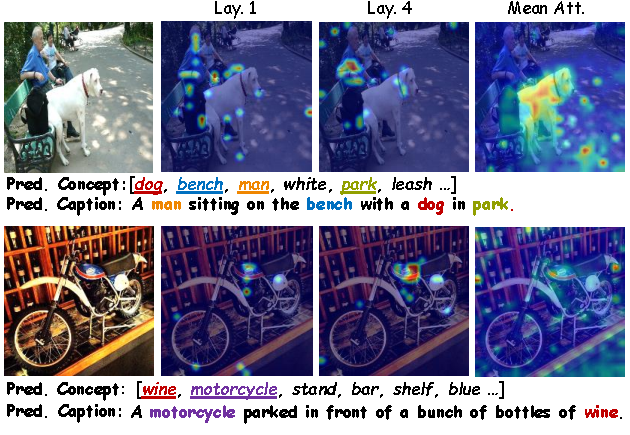
\includegraphics[width=.86\textwidth]{images/main_qualitative.pdf}
  \end{center}
  \vspace{-6mm}
    \caption[Visualization of the attention maps from \vitcapp and its produced concepts\&captions.]{\small Visualization of the attention maps from \vitcapp and its produced concepts\&captions. ``\rule{6mm}{0.15mm}'' refers to the concepts appear in captions. Best viewed in colors.
    }
    \vspace{-4mm}
  \label{fig:qualitative}
\end{figure}



\vspace{1mm}
\noindent \textbf{Qualitative Examples.} We show visualization examples of the attention maps from \vitcap in Figure~\ref{fig:qualitative} together with their generated concepts\&captions. Interestingly, we observe obvious correlations between the attended regions across different layers and predicted concepts. For example, ``{\color{black} \texttt{\textbf{dog}}}'' is notably highlighted according to the mean-averaged attention maps, yet the ``{\color{black} \texttt{\textbf{man}}}'' is more attended in shallower transformer blocks. We conjecture that instead of relying on an object detector to glean object locations, training the detector-free VL model properly via image-text supervisions might potentially lead to a strong grounding model as a promising future endeavor. 



\begin{figure}[t!]
    \centering
    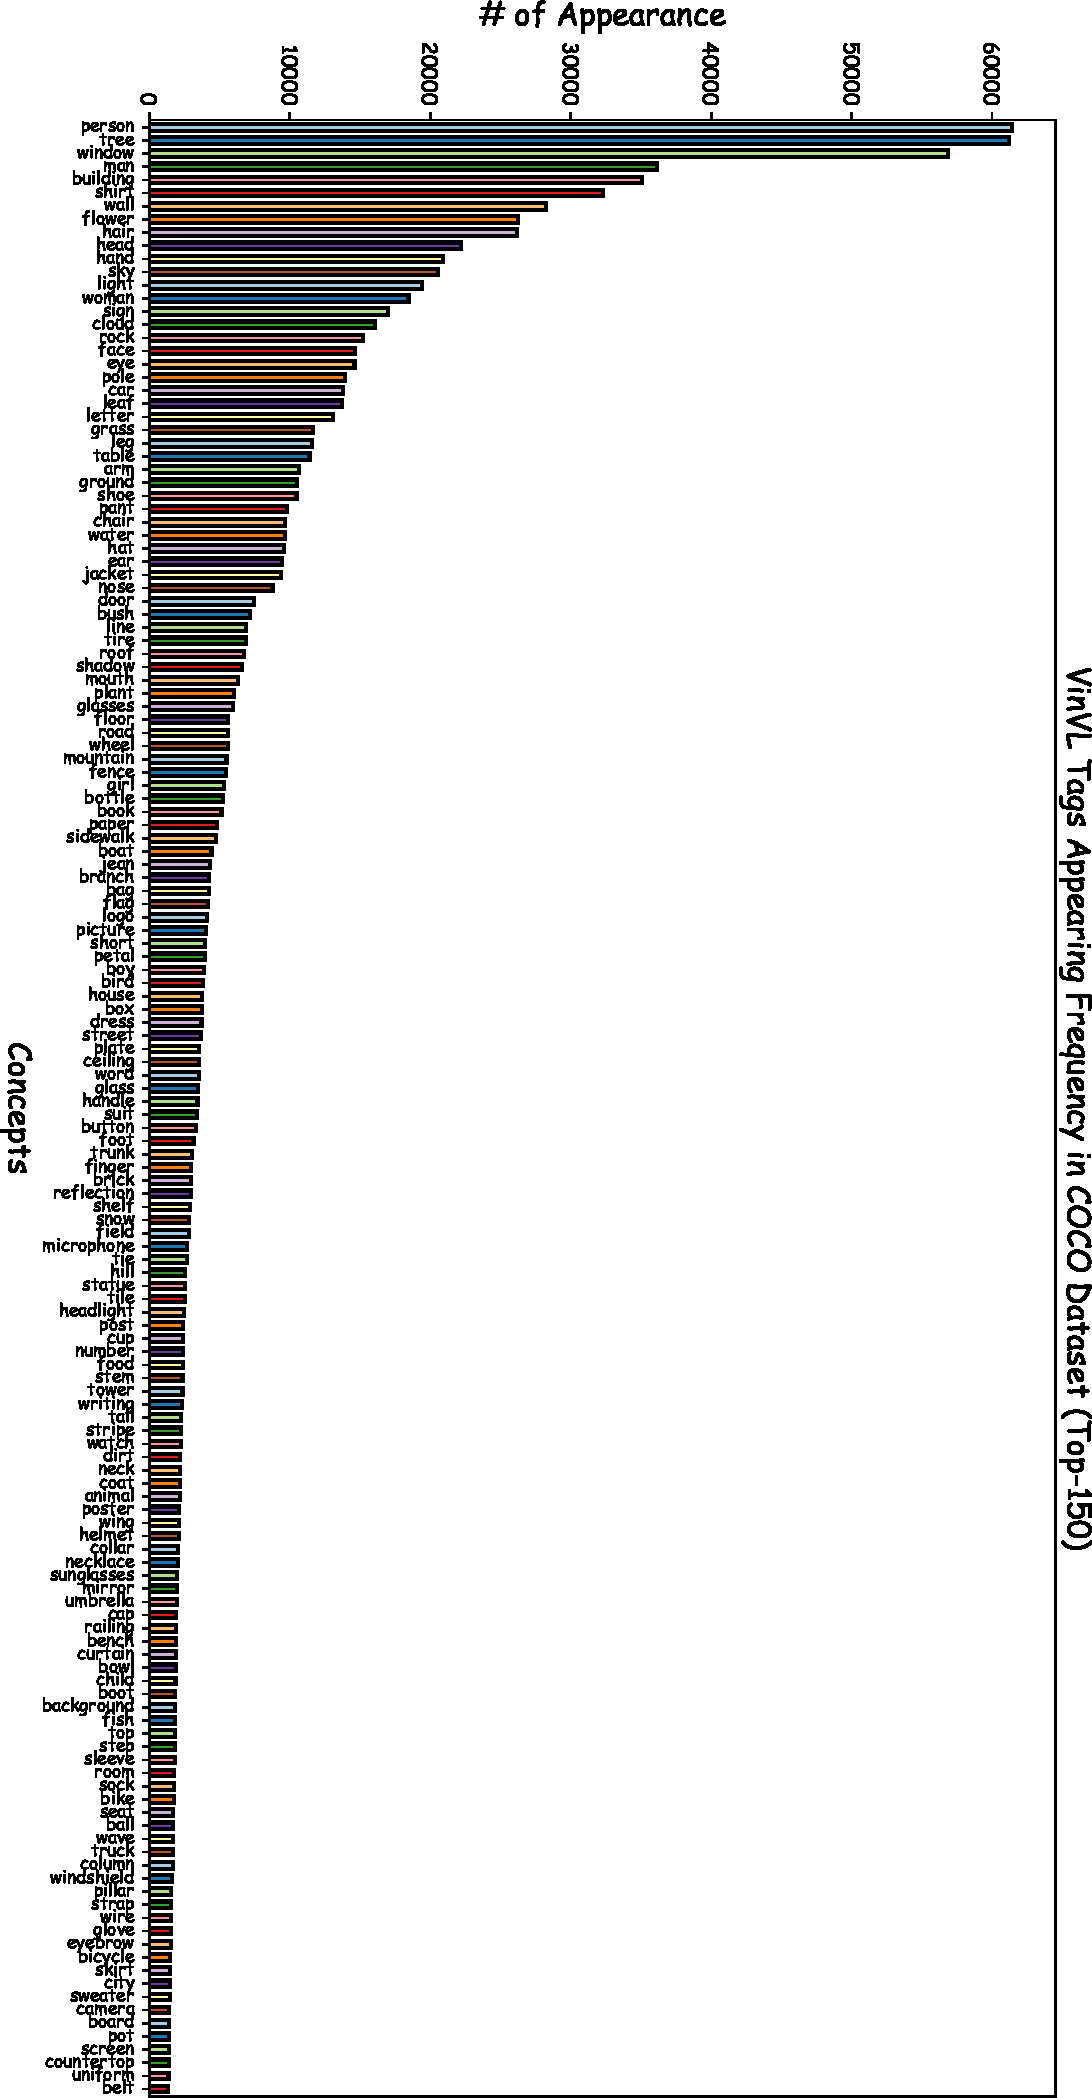
\includegraphics[width=.7\linewidth]{images/stats_rotated.pdf}
    \caption[Top-$150$ most frequently appeared semantic concepts produced by VinVL's object detector.]{Top-$150$ most frequently appeared semantic concepts produced by VinVL's object detector. The produced tags are severely long-tail distributed and certain concepts dominates across all samples. This arises the necessity to apply focal loss as countermeasure. }
    \label{fig:stats}
\end{figure}



  
 
\begin{table}[t!]
\begin{center}
\caption{Statistics of the VL pre-training datasets. }
\begin{tabular}{c@{\hspace{3pt}}|c@{\hspace{3pt}}|c|c|c@{\hspace{3pt}}}
\toprule
Source & VG & COCO & CC& SBU\\
\midrule
Image & 108K & 113K & 3.1M & 875K  \\
Text & 5.4M & 567K & 3.1M & 875K  \\
\bottomrule
\end{tabular}
\end{center}
\label{tab:vlcorpus}
\end{table}


\subsubsection{Pre-training VL Corpus}
As previous works in~\citep{zhang2021multi}, we carry out the pre-training of ViTCAP on the aggregation of several common datasets, which include COCO~\citep{lin2014microsoft}, Conceptual Caption~\citep{changpinyo2021conceptual}, SBU Captions~\citep{ordonez2011im2text}, and Visual Genome~\citep{krishna2017visual}. We have the detailed statistics of the aggregated datasets in the above Table. In total, we use $4.2$ millions images and $9.9$M captions for the pre-training. Following~\citep{lu202012}, we de-duplicate images exist in both pre-training corpus and COCO Karpathy testing splits for fair comparisons.



\subsubsection{Ablative Studies}
This section further presents additional ablative studies about ViTCAP, which includes: some examples and basic statistics about semantic concepts, effect of differnet concept sources, 
results of different concept classification losses, different other training strategies.



\vspace{1mm}
\noindent\textbf{Examples and Stats of Concepts.}
In practice, we experiment with utilizing semantic concepts gleaned from 1). open-form image captions by language parsing (or simple as using all tokens as classification ground-truth) or 2).  an object detector. 

As previously mentioned, we notice that the concepts from both sides are all severely long-tailed distributed (an example of the detector-produced concept distribution is shown in Figure~\ref{fig:stats}). Notably, certain concepts appear more frequently across the whole COCO training split, \eg, ``\texttt{person}'', ``\texttt{tree}'', ``\texttt{window}'' obviously exist far more frequent than the remaining.  We also resort to different object detectors to acquire high-quality semantic concepts, \ie, a ResNet$_{101}$ base Faster-RCNN~\citep{anderson2018bottom} that has been pre-trained on Visual-Genome dataset~\citep{krishna2017visual} (denoted as BUTD), and a ResNext$_{152}$ based modified Faster-RCNN detector with broader categories of the visual attribute as detection targets (denoted as VinVL). These detector-produced image-level tags are actually accurate with less noise as in captions, but they also require the pre-defined categorical dictionary with fixed set of concepts. This largely limits the scope of their applications.

\vspace{1mm}
\noindent\textbf{More About Concept Sources.}
Open-form captions are the most idea source to obtain semantic concepts as they naturally carry abundant semantic concepts with no vocabulary limitation. Notwithstanding that most of these descriptions can be noisy, inaccurate and incomplete. In practice, we leverage different ways to extract the concepts from them by 1) using the NLTK~\citep{loper2002nltk} toolkit and parse out only the nouns and adjectives as the semantic concepts for the classification task (see ``CAPTION'' baseline in main paper); 2) we also simply attempt to leverage all tokens from the captions as concept targets in case of omitting essential words during parsing (see ``$^{\spadesuit}$'' in main paper).
We first extract these tags as ``\textit{off-the-shelf}'' annotations for the concept classification task and then apply the initialization of VitCAP after first stage training for the joint captioning training. Note that we conduct and compare all these ablations without VL pre-training. It is beneficial to further adopt the concept classification loss during the joint training, as the semantic concepts in the COCO-caption dataset vary with the concept classification dataset. Also, captions in these two domains might vary from the aspect of textual styles: for example, length of captions, the use of synonym, cognate and conjugate words or various tenses.



\begin{table}[h]
\centering
\setlength{\tabcolsep}{4pt} % Default value: 6pt
\renewcommand{\arraystretch}{1.15} % Default value: 1
\caption{\small Performances of ViTCAP using focal loss, binary classification loss as concept classification training target. 
}
% \vspace{-2mm}
\scalebox{0.99}{
 \small
\begin{tabular}{l|c|ccccc}
\toprule
 & \multicolumn{5}{c}{{ \texttt{\textbf{COCO Captioning}}}}  \\ 
& EPOCH & {B@4} & {M} & {R} & {C} & {S} \\
\hline 
%  {\transparent{0.4} Baseline$_{32\times32}$} & {\transparent{0.4} -} & {\transparent{0.4} $33.9$} &
  {\transparent{0.4} Baseline} & {\transparent{0.4} -} & {\transparent{0.4} $33.9$} &
  {\transparent{0.4} $27.8$} &  {\transparent{0.4} $56.4$} & {\transparent{0.4} $114.8$} &  {\transparent{0.4} $21.3$} \\
 {\transparent{0.4} VinVL-Tag} & {\transparent{0.4} -} & {\transparent{0.4} $35.4$} & {\transparent{0.4} $28.1$} &  {\transparent{0.4} $57.2$} & {\transparent{0.4} $117.7$} &  {\transparent{0.4} $21.3$} \\
\hline
% BCE$_\text{Tag}$  & $10$ & \\ 
BCE$_\text{Tag}$  & $10$ & $33.9$ & $27.9$ & $56.5$ & $115.0$ & $21.4$\\ 
FOCAL$_\text{Tag}$ & $10$ & $35.2$ & $28.0$ & $57.0$ & $117.1$ & $21.4$\\ 
FOCAL$_\text{Tag+Init}$ & $10$ & $36.0$ & $28.4$ & $57.5$ & $120.5$ & $22.0$\\ 
FOCAL$_\text{Init}$ & $10$ & $35.0$ & $28.2$ & $57.1$ & $118.0$ & $21.6$\\ 
FOCAL$_\text{Tag+Init}$ & $40$ & $35.9$ & $28.4$ & $57.6$ & $121.1$ & $22.1$ \\ 
\bottomrule
\end{tabular}
}
\label{tab:losses}
\end{table} 

\vspace{1mm}
\noindent\textbf{Concept Classification Training.}
We now study the effect of different losses for the concept classification task, namely binary cross-entropy loss and the focal loss and the effect of the initialization after the classification training. 
The extremely imbalanced sample distribution usually lead to sub-optimal classification performances, as also studied in previous works like face recognition~\citep{zhang2017range,ma2020learning} and object detection~\citep{li2020overcoming, ouyang2016factors}, etc. As countermeasures, there exist works designing advanced losses~\citep{lin2017focal,zhang2017range} re-weighting different samples. In Table~\ref{tab:losses}, we list the performances of ViTCAP using different losses. In specific, the top-two rows are the baseline results 1). Baseline: vanilla Encoder-Decoder architecture without CTN branch, and 2). Encoder-Decoder architecture using VinVL's OD tags as~\citep{li2020oscar}. ``$_\text{Tag}$'' denotes the results are reported using concepts as the offline tags without concept classification \& its initialization. We observe that by applying the BCE loss trained offline concepts as offline tags, the results are only incrementally improved over the baseline, and it still shows a great performance gap \textit{w.r.t.} the VinVL's tag. Notably, using focal loss obviously improves the quality of produced concepts, reaching $117.1$ CIDEr scores. To this end, we apply the concept classification pre-trained initialization, and this
further improves the performances to a great extent. It is discernible that the experiment ``$_\text{Init}$'' gives worse result than the ``$_\text{Tag+Init}$''. This validates that both the concept classification task and the predicted concepts are helpful for the captioning task. Results show that they are complementary to each other.


\begin{table}[h]
\centering
\setlength{\tabcolsep}{4pt} % Default value: 6pt
\renewcommand{\arraystretch}{1.15} % Default value: 1
\caption{\small Performances of VitCAP using different strategies for concept tokenization. 
}
% \vspace{-2mm}
\scalebox{0.99}{
 \small
\begin{tabular}{l|ccccc}
\toprule
\multirow{2}{*}{Tokenization} & \multicolumn{5}{c}{{ \texttt{\textbf{COCO Captioning}}}}  \\ 
 & {B@4} & {M} & {R} & {C} & {S} \\
\hline 
Caption Tokenizer & $35.5$ & $28.5$ & $57.5$ & $119.7$ & $21.8$ \\ 
Classifier Tokenizer & $35.6$ & $28.4$ & $57.4$ & $119.8$ & $21.8$ \\ 
Independent Tokenizer & $35.9$ & $28.5$ & $57.6$ & $120.1$ & $21.9$ \\ 
\bottomrule
\end{tabular}
}
\label{tab:tokenizer}
\end{table} 

\noindent\textbf{Representing Concepts as Tokens.} There are multiple ways to encode the predicted concepts as continuous embedding for decoding stage. We study three different ways of encoding and present the results in Table~\ref{tab:tokenizer}, namely, 1). use the tokenizer for captioning, 2). use the concept classifier's tokenizer (in concept classification, we simply use the BERT tokenizer to encode the semantic concepts), 3). use an independent and untrained tokenizer. Though in practice, all three tokenizers are implemented based on the BERT tokenizer~\citep{devlin2018bert}, the embeddings from the three are entirely different. From the results, we observe fairly negligible performance gap: using independent tokenizer only yields $0.4$ higher CIDEr score. Though adopting an independent tokenizer yields the best result, it introduces additional parameters and thus we choose to share the tokenizer for captioning instead. 


% \section{More Details about Training\&Evaluation}


\begin{table}[h]
\centering
\setlength{\tabcolsep}{4pt} % Default value: 6pt
\renewcommand{\arraystretch}{1.15} % Default value: 1
\caption{\small Performances of ViTCAP using either ground-truth concepts for captioning, the concept network predicted concept tokens, or the mixed of them during training. 
}
% \vspace{-2mm}
\scalebox{0.99}{
 \small
\begin{tabular}{l|ccccc}
\toprule
\multirow{2}{*}{\textbf{}} & \multicolumn{5}{c}{{ \texttt{\textbf{COCO Captioning}}}}  \\ 
& {B@4} & {M} & {R} & {C} & {S} \\
\hline 
GT Concepts & $35.5$ & $28.4$ & $57.3$ & $119.1$ & $21.7$ \\ 
GT + PRED. Concepts & $35.2$ & $28.5$ & $57.3$ & $119.2$ & $21.8$\\ 
PRED. Concepts & $36.1$ & $28.6$ & $57.6$ & $120.6$ & $21.7$\\ 
\bottomrule
\end{tabular}
}
\label{tab:concept}
\end{table} 

We experiment with different ways to train with the concept tokens. In Table~\ref{tab:concept}, we list results of training using GT semantic concepts encoded as tokens, GT concepts mixed with predicted concepts, and fully predicted concepts.

\begin{figure*}[h!]
  \begin{center}
    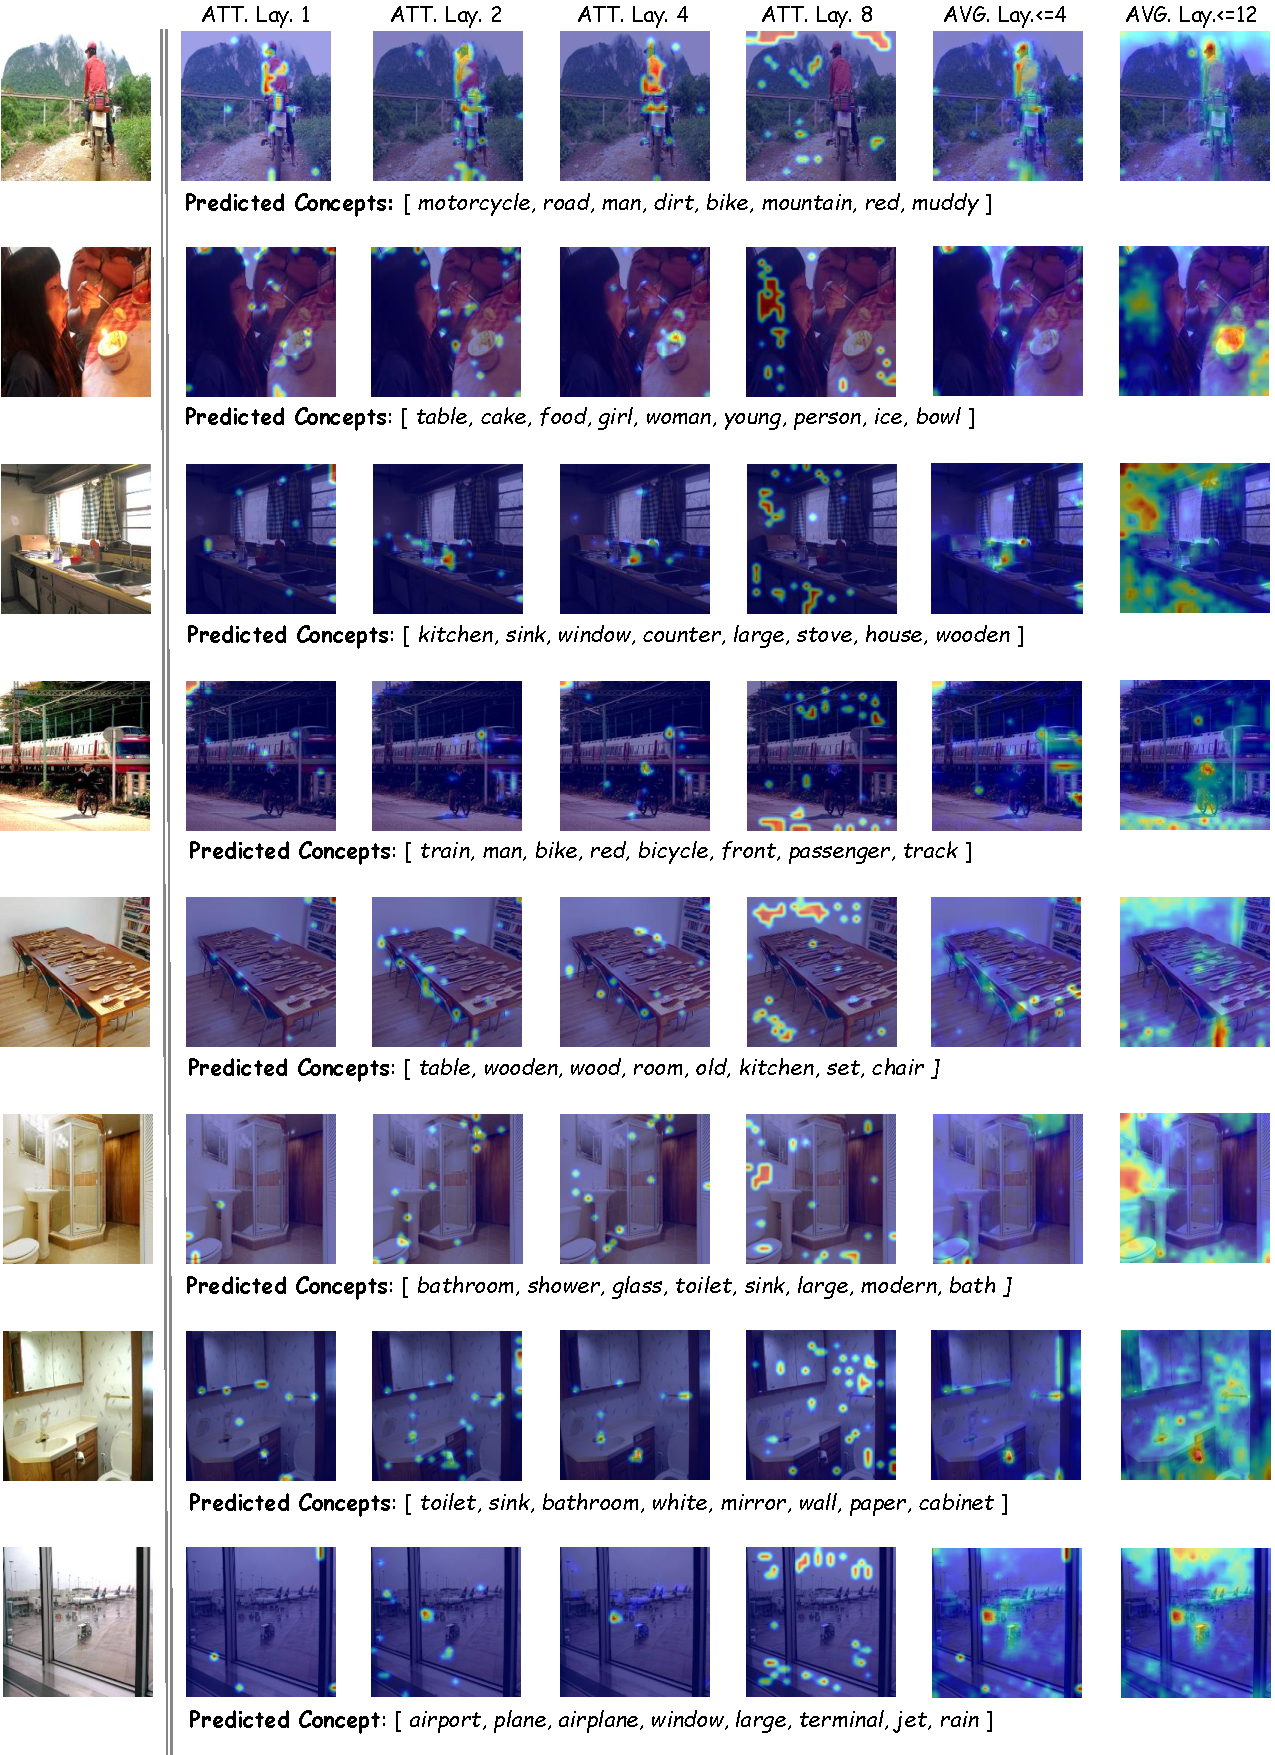
\includegraphics[width=0.9\textwidth]{./images/vitcap_qualitative.pdf}
    \vspace{-6mm}
  \end{center}
    \caption[ViTCAP produced class-agnostic attention maps and their associated semantic concepts of random images from COCO caption dataset. ]{\small ViTCAP produced class-agnostic attention maps and their associated semantic concepts of random images from COCO caption dataset. We exhibit attention maps of $1$, $2$, $4$, $8$th transformer blocks of ViTCAP and the mean-average attention maps of first $4$ and the entire $12$ transformer blocks (last two columns).
    }
  \label{fig:qualitative}
\end{figure*}

We find that by using the predicted concepts for training lead to optimal results. This is mostly because that the pre-trained CTN can already produce reasonable concepts at the captioning fine-tuning stage. 


\begin{table}[h]
\centering
\setlength{\tabcolsep}{6pt} % Default value: 6pt
\renewcommand{\arraystretch}{1.15} % Default value: 1
% \vspace{-2mm}
\caption[We compare different instantiations of ViTCAP with architectural variations of ViT based captioning model.]{\small
We compare different instantiations of VitCAP with architectural variations of ViT based captioning model: single-tower (SIN-TOW), encoder-decoder structure (ENC-DEC), two-tower ViTCAP, and ViTCAP with various numbers of sharing blocks in stem image encoder. All experiments are conducted without VL pre-training and are trained by cross-entropy loss.
}
\scalebox{0.99}{
 \small
\begin{tabular}{l|ccccc}
\toprule
\multirow{2}{*}{\textbf{Architecture}} & \multicolumn{5}{c}{{ \texttt{\textbf{COCO Captioning}}}}  \\ 
& {B@4} & {M} & {R} & {C} & {S} \\
\hline 
SIN-TOW$_{32\times32}$ & $32.5$ & $27.1$ & $55.4$ & $109.5$ & $20.2$ \\ 
$_{+\text{EFF. OD-Tags}}$ & $32.8$ &  $27.4$ & 	$55.5$ & $110.9$ &	$20.6$ \\
$_{+\text{VinVL-Tags}}$ &  $33.5$ & $27.8$ & $56.1$ & $114.6$ & $21.1$\\
\hline
ENC-DEC$_{32\times32}$ & $33.4$ & $27.5$ & $56.0$ & $112.1$ & $20.6$ \\
$_{+\text{EFF. OD-Tags}}$ & $33.8$ & $27.9$ & $56.4$ & $114.6$ & $21.3$  \\
$_{+\text{VinVL-Tags}}$ & $34.4$ & 	$27.9$ & $56.6$ & $115.8$& $21.1$\\
$_{+\text{ViTCAP-Tags}}$ & $34.0$ &	$27.7$ & $56.3$ & $114.2$ & $20.8$\\
\hline
SIN-TOW$_{16\times16}$ & $33.8$ & $27.8$ &	$56.2$ & $113.9$ & $21.0$\\ 
$_{+\text{EFF. OD-Tags}}$ & $33.8$ & $27.9$  &	$56.4$ &	$114.6$ &	$21.3$ \\
$_{+\text{VinVL-Tags}}$ &  $34.3$ &	$28.2$ & $56.7$ & $117.4$	& $21.7$ \\
\hline
ENC-DEC$_{16\times16}$ & $33.9$ &$27.8$ &	$56.4$ &	$114.8$ &	$21.3$ \\
$_{+\text{VinVL-Tags}}$ &  $35.4$ &	$28.1$ & $57.2$ & 	$117.7$ &	$21.3$\\
$_{+\text{ViTCAP-Tags}}$  & $35.2$ & 	$28.0$ & 	$57.0$	 & $117.1$ & 	$21.4$\\
\hline
ViTCAP\\
$M_1=8$ &  $36.3$ &   $28.9$ &   $57.7$ & $123.0$ &    $22.1$\\
$M_1=4$ & $36.1$ &   $28.8$ &   $57.6$ & $122.2$ &    $22.1$\\
\bottomrule
\end{tabular}
}
\label{tab:arch}
\end{table} 



\begin{figure}[t]
%  \vspace{-3mm}
  \begin{center}
  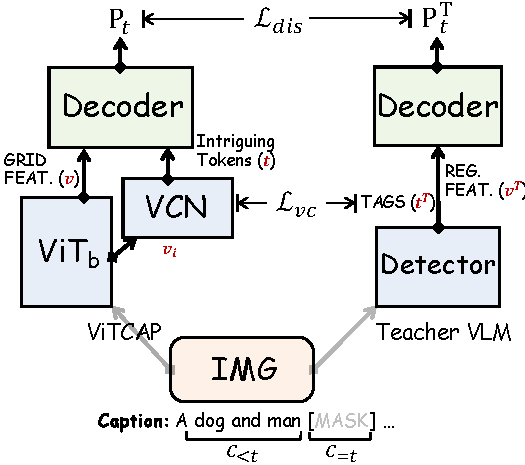
\includegraphics[width=.76\textwidth]{./images/distillation.pdf}
  \end{center}
  \vspace{-6mm}
    \caption[The overall training paradigm of ViTCAP.]{\small The overall training paradigm of ViTCAP can be understood as the knowledge distillation procedure where a detector-based Teacher VLM to assist the training of ViTCAP as a knowledge distillation paradigm. The CTN branch in ViTCAP learns to predict the semantic concepts as conceptual tokens for captioning. }
    \vspace{-2mm}
  \label{fig:distillation}
\end{figure}


\vspace{1mm}
\noindent \textbf{ViTCAP Architecture.} To give a more detailed explanation about the architecture of ViTCAP: it is consisted of a stem image encoder with $8$ transformer blocks (shared for both grid feature extractor and CTN), a CTN branch with $4$ transformer blocks, and a grid feature extractor with $4$ transformer blocks, the multi-modal module is also a $4$ transformer blocks module. When $M_1=12$, the model can be understood as consisting of two parallel branches, with one for concept prediction and one for grid representation. We does find that minimizing the shared blocks can bring extra performance gains but this inevitably increases the model size very obviously.
More experiments about different architectural instantiations are provided in the following.


\vspace{1mm}
\noindent \textbf{Architectural Variations.} We then experiment
with different architectural variations of ViTCAP and report their performances on COCO-caption in Table~\ref{tab:arch}. 
The baseline models include single-tower (SIN-TOW) that shares the ViT backbone for both modalities; Encoder-decoder (ENC-DEC) that use a ViT as visual encoder and 4 separate transformer blocks as modal fusion. This is similar to~\citep{kim2021vilt}, however we modify it with using seq-to-seq attention maps for the captioning training which prevents the model from seeing bidirectional context; Two-tower (TWO-TOW) uses an independent ViT/b architecture as conceptual token network and another architecture as the visual encoder; And VitCAP with different number of sharing blocks. We attach detailed architectures for these variations in the later section together with their learnable parameters. When adopting $8$ transformer blocks in the stem image encoder, we observe VitCAP achieves the close performances when $M_1=4$.



\vspace{1mm}
% \noindent\textbf{Evaluations on Google-CC and nocaps.}


% \section{Qualitative Examples}


\subsection{Discussions}
\noindent\textbf{Qualitative Examples.}
We demonstrate more qualitative examples of the attention maps produced by VitCAP together with their predicted semantic concepts in Figure~\ref{fig:qualitative}. 

\vspace{1mm}
\noindent\textbf{Can ViTCAP Ground Concepts?} Interestingly, we observe that the attention maps produced from transformer blocks closely relate to the concepts and various layers have different focuses while the averaged attention maps cover a broad holistic regions. We present more visualizations in Figure~\ref{fig:grounding} which contain single object per image for more direct analysis. The topmost row is a picture with multiple ``\texttt{wild gooses}'' and all regions of them are highlighted according to the attention maps. Despite so, it seems VitCAP suffers from identifying the clear borders of the object that it may only recognize part of the objects, \eg, ViTCAP only highlights the part of the ``\texttt{traffic light}'' and the ``\texttt{tie}''.

\vspace{1mm}
\noindent\textbf{VL Distillation Schema.} Our distillation schema can be indeed viewed as an extension of the VL distillation schema, where the Student model not only mimic the predicted masked token probability but also learns from the Teacher OD's object tags. As is shown in Figure~\ref{fig:distillation}. Note that our distillation technique is only applied on the \vitcap with VL pre-training, as the teacher VL model contains knowledge acquired from large scale pre-training and so it is unfair to compare the \vitcap with other methods without VL pre-training.

\begin{figure*}[t!]
%  \vspace{-3mm}
  \begin{center}
  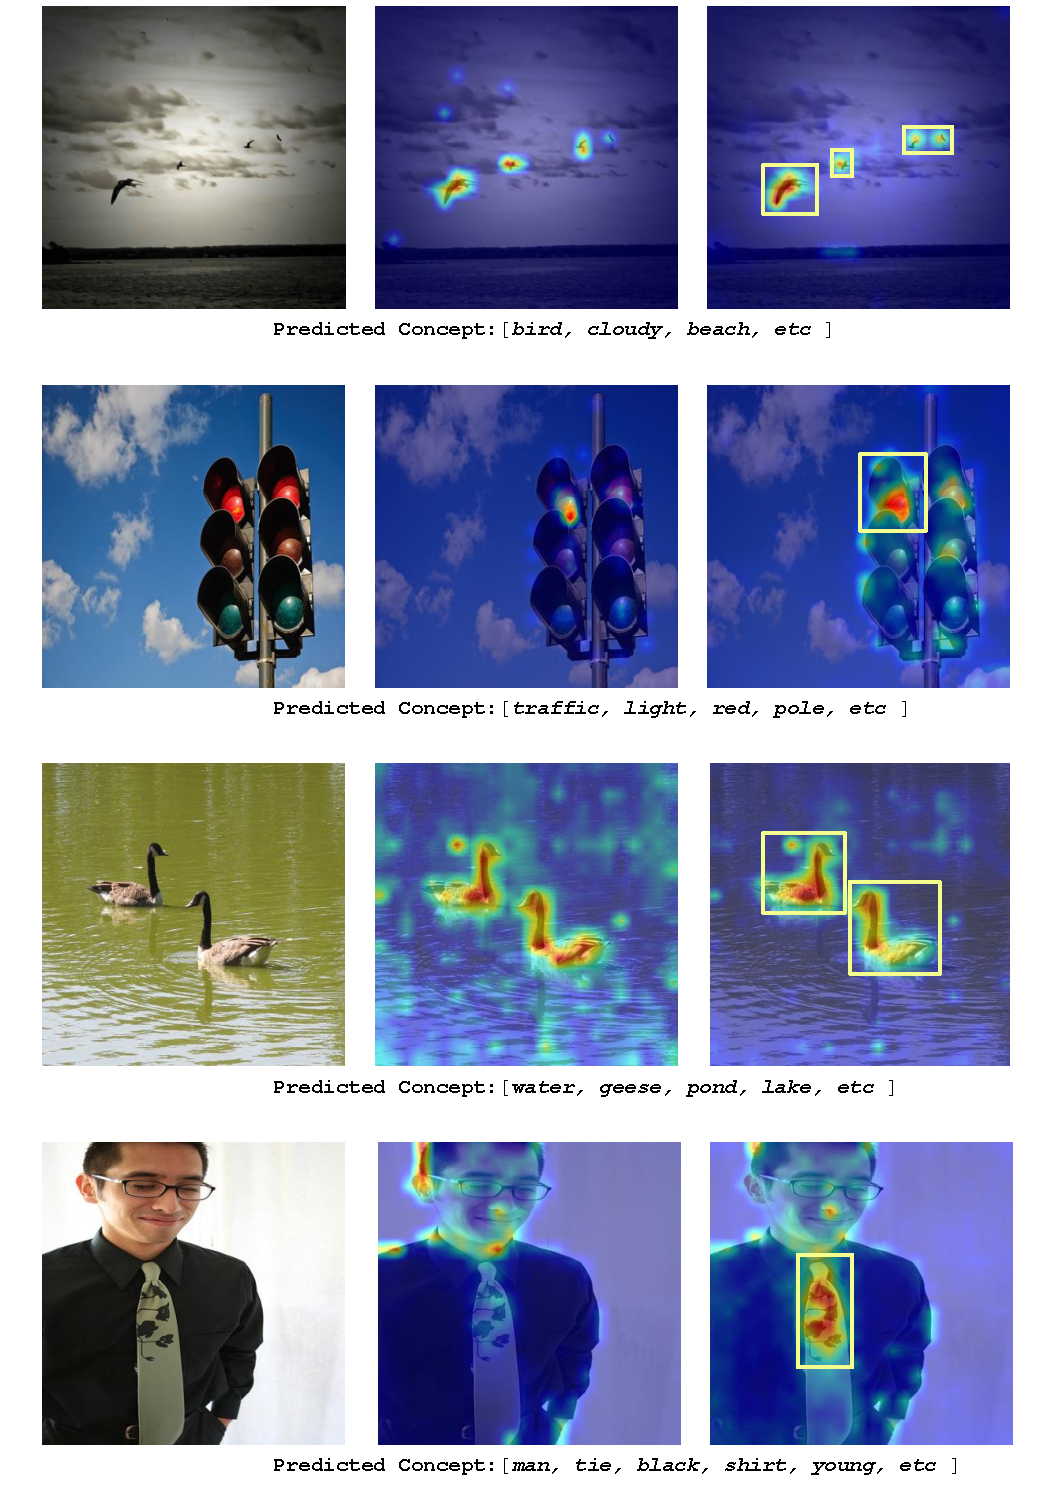
\includegraphics[width=.75\textwidth]{./images/grounding.pdf}
  \end{center}
  \vspace{-6mm}
    \caption{\small From left to right, we show the original image, average attention maps of the front 4 and 8 transformer blocks.  }
    \vspace{-2mm}
  \label{fig:grounding}
\end{figure*}



\vspace{1mm}
\noindent\textbf{Detector Tags \vs Caption Extracted Concepts.} Empirical studies show that the caption extracted concepts lead to better \vitcap\!. We conjecture that this is mainly because that the captions contain much broader image concepts contained in open-form texts, yet the detector tags are pre-defined with much more limited vocabulary. However, perfectly aligned image-text pairs are not always attainable considering that most existing image-level annotations are collected from Web. These image captions can be as noisy as alt text or short phrases, from which the extracted concepts only cover partial of the image content. Thus in practice, it is also an important aspect to explore the feasibility of adopting the non caption-extracted concepts, \eg, from an object detector as substitution. This provides a flexible source of the concepts. 




\subsection{Conclusion}
In this paper, we propose the ViTCAP, a detector-free image captioning model in the full transformer fashion. Compared with prior arts, \vitcap can be trained in an end-to-end fashion without intermediate regional operations using grid representations. Our proposed Concept Token Network learns broad semantic concepts and encodes them as the concept tokens that largely benefit the captioning task on a series of challenging captioning benchmarks. Extensive experiments indicate that \vitcap achieves competing performances, approaching most detector-based models. 

\vspace{-2mm}
